%% LyX 2.3.7 created this file.  For more info, see http://www.lyx.org/.
%% Do not edit unless you really know what you are doing.
\documentclass[journal,article,submit,pdftex,moreauthors]{Definitions/mdpi}
\usepackage[utf8]{inputenc}
\usepackage{float}
\usepackage{url}
\usepackage{amsmath}
\usepackage{graphicx}

\makeatletter

%%%%%%%%%%%%%%%%%%%%%%%%%%%%%% LyX specific LaTeX commands.

\Title{Training neural networks with a procedure guided by BNF grammars}

\TitleCitation{Training neural networks with a procedure guided by BNF grammars}

\Author{Ioannis G. Tsoulos$^{1,*}$, Vasileios Charilogis$^{2}$}

\AuthorNames{Ioannis G. Tsoulos, Vasileios Charilogis}

\AuthorCitation{Tsoulos, I.G.; Charilogis, V.}


\address{$^{1}$\quad{}Department of Informatics and Telecommunications,
University of Ioannina, Greece; itsoulos@uoi.gr\\
$^{2}$\quad{}Department of Informatics and Telecommunications, University
of Ioannina, Greece; v.charilog@uoi.gr}


\corres{Correspondence: itsoulos@uoi.gr}


\abstract{Artificial neural networks are parametric machine learning models
that have been applied successfully to an extended series of classification
and regression problems found in the recent literature. For the effective
identification of the parameters of the artificial neural networks,
a series of optimization techniques have been proposed in the relevant
literature, which, although they present good results in many cases,
either the optimization method used is not efficient and the training
error of the network is trapped in sub-optimal values, or the neural
network exhibits the phenomenon of over-training which means that
it has poor results when applied to data that was not present during
the training. This paper proposes an innovative technique for constructing
the weights of artificial neural networks based on appropriate BNF
grammars, used in the evolutionary process of Grammatical Evolution.
The new procedure locates an interval of values for the parameters
of the artificial neural network, and the optimization method effectively
locates the network parameters within this interval. The new technique
was applied to a wide range of data classification and adaptation
problems covering a number of scientific areas and the experimental
results were more than promising.}


\keyword{Neural networks; Genetic algorithms; Grammatical Evolution; Evolutionary
algorithms}

\DeclareTextSymbolDefault{\textquotedbl}{T1}
%% Because html converters don't know tabularnewline
\providecommand{\tabularnewline}{\\}
\floatstyle{ruled}
\newfloat{algorithm}{tbp}{loa}
\providecommand{\algorithmname}{Algorithm}
\floatname{algorithm}{\protect\algorithmname}

%%%%%%%%%%%%%%%%%%%%%%%%%%%%%% Textclass specific LaTeX commands.
\newenvironment{lyxcode}
	{\par\begin{list}{}{
		\setlength{\rightmargin}{\leftmargin}
		\setlength{\listparindent}{0pt}% needed for AMS classes
		\raggedright
		\setlength{\itemsep}{0pt}
		\setlength{\parsep}{0pt}
		\normalfont\ttfamily}%
	 \item[]}
	{\end{list}}

%%%%%%%%%%%%%%%%%%%%%%%%%%%%%% User specified LaTeX commands.
%  LaTeX support: latex@mdpi.com 
%  For support, please attach all files needed for compiling as well as the log file, and specify your operating system, LaTeX version, and LaTeX editor.

%=================================================================


% For posting an early version of this manuscript as a preprint, you may use "preprints" as the journal and change "submit" to "accept". The document class line would be, e.g., \documentclass[preprints,article,accept,moreauthors,pdftex]{mdpi}. This is especially recommended for submission to arXiv, where line numbers should be removed before posting. For preprints.org, the editorial staff will make this change immediately prior to posting.

%--------------------
% Class Options:
%--------------------
%----------
% journal
%----------
% Choose between the following MDPI journals:
% acoustics, actuators, addictions, admsci, adolescents, aerospace, agriculture, agriengineering, agronomy, ai, algorithms, allergies, alloys, analytica, animals, antibiotics, antibodies, antioxidants, applbiosci, appliedchem, appliedmath, applmech, applmicrobiol, applnano, applsci, aquacj, architecture, arts, asc, asi, astronomy, atmosphere, atoms, audiolres, automation, axioms, bacteria, batteries, bdcc, behavsci, beverages, biochem, bioengineering, biologics, biology, biomass, biomechanics, biomed, biomedicines, biomedinformatics, biomimetics, biomolecules, biophysica, biosensors, biotech, birds, bloods, blsf, brainsci, breath, buildings, businesses, cancers, carbon, cardiogenetics, catalysts, cells, ceramics, challenges, chemengineering, chemistry, chemosensors, chemproc, children, chips, cimb, civileng, cleantechnol, climate, clinpract, clockssleep, cmd, coasts, coatings, colloids, colorants, commodities, compounds, computation, computers, condensedmatter, conservation, constrmater, cosmetics, covid, crops, cryptography, crystals, csmf, ctn, curroncol, currophthalmol, cyber, dairy, data, dentistry, dermato, dermatopathology, designs, diabetology, diagnostics, dietetics, digital, disabilities, diseases, diversity, dna, drones, dynamics, earth, ebj, ecologies, econometrics, economies, education, ejihpe, electricity, electrochem, electronicmat, electronics, encyclopedia, endocrines, energies, eng, engproc, ent, entomology, entropy, environments, environsciproc, epidemiologia, epigenomes, est, fermentation, fibers, fintech, fire, fishes, fluids, foods, forecasting, forensicsci, forests, foundations, fractalfract, fuels, futureinternet, futureparasites, futurepharmacol, futurephys, futuretransp, galaxies, games, gases, gastroent, gastrointestdisord, gels, genealogy, genes, geographies, geohazards, geomatics, geosciences, geotechnics, geriatrics, hazardousmatters, healthcare, hearts, hemato, heritage, highthroughput, histories, horticulturae, humanities, humans, hydrobiology, hydrogen, hydrology, hygiene, idr, ijerph, ijfs, ijgi, ijms, ijns, ijtm, ijtpp, immuno, informatics, information, infrastructures, inorganics, insects, instruments, inventions, iot, j, jal, jcdd, jcm, jcp, jcs, jdb, jeta, jfb, jfmk, jimaging, jintelligence, jlpea, jmmp, jmp, jmse, jne, jnt, jof, joitmc, jor, journalmedia, jox, jpm, jrfm, jsan, jtaer, jzbg, kidney, kidneydial, knowledge, land, languages, laws, life, liquids, literature, livers, logics, logistics, lubricants, lymphatics, machines, macromol, magnetism, magnetochemistry, make, marinedrugs, materials, materproc, mathematics, mca, measurements, medicina, medicines, medsci, membranes, merits, metabolites, metals, meteorology, methane, metrology, micro, microarrays, microbiolres, micromachines, microorganisms, microplastics, minerals, mining, modelling, molbank, molecules, mps, msf, mti, muscles, nanoenergyadv, nanomanufacturing, nanomaterials, ncrna, network, neuroglia, neurolint, neurosci, nitrogen, notspecified, nri, nursrep, nutraceuticals, nutrients, obesities, oceans, ohbm, onco, oncopathology, optics, oral, organics, organoids, osteology, oxygen, parasites, parasitologia, particles, pathogens, pathophysiology, pediatrrep, pharmaceuticals, pharmaceutics, pharmacoepidemiology, pharmacy, philosophies, photochem, photonics, phycology, physchem, physics, physiologia, plants, plasma, pollutants, polymers, polysaccharides, poultry, powders, preprints, proceedings, processes, prosthesis, proteomes, psf, psych, psychiatryint, psychoactives, publications, quantumrep, quaternary, qubs, radiation, reactions, recycling, regeneration, religions, remotesensing, reports, reprodmed, resources, rheumato, risks, robotics, ruminants, safety, sci, scipharm, seeds, sensors, separations, sexes, signals, sinusitis, skins, smartcities, sna, societies, socsci, software, soilsystems, solar, solids, sports, standards, stats, stresses, surfaces, surgeries, suschem, sustainability, symmetry, synbio, systems, taxonomy, technologies, telecom, test, textiles, thalassrep, thermo, tomography, tourismhosp, toxics, toxins, transplantology, transportation, traumacare, traumas, tropicalmed, universe, urbansci, uro, vaccines, vehicles, venereology, vetsci, vibration, viruses, vision, waste, water, wem, wevj, wind, women, world, youth, zoonoticdis 

%---------
% article
%---------
% The default type of manuscript is "article", but can be replaced by: 
% abstract, addendum, article, book, bookreview, briefreport, casereport, comment, commentary, communication, conferenceproceedings, correction, conferencereport, entry, expressionofconcern, extendedabstract, datadescriptor, editorial, essay, erratum, hypothesis, interestingimage, obituary, opinion, projectreport, reply, retraction, review, perspective, protocol, shortnote, studyprotocol, systematicreview, supfile, technicalnote, viewpoint, guidelines, registeredreport, tutorial
% supfile = supplementary materials

%----------
% submit
%----------
% The class option "submit" will be changed to "accept" by the Editorial Office when the paper is accepted. This will only make changes to the frontpage (e.g., the logo of the journal will get visible), the headings, and the copyright information. Also, line numbering will be removed. Journal info and pagination for accepted papers will also be assigned by the Editorial Office.

%------------------
% moreauthors
%------------------
% If there is only one author the class option oneauthor should be used. Otherwise use the class option moreauthors.

%---------
% pdftex
%---------
% The option pdftex is for use with pdfLaTeX. If eps figures are used, remove the option pdftex and use LaTeX and dvi2pdf.

%=================================================================
% MDPI internal commands - do not modify
\firstpage{1} 
 
\setcounter{page}{\@firstpage} 

\pubvolume{1}
\issuenum{1}
\articlenumber{0}
\pubyear{2024}
\copyrightyear{2024}
%\externaleditor{Academic Editor: Firstname Lastname} % For journal Automation, please change Academic Editor to "Communicated by"
\datereceived{}
\daterevised{ } % Comment out if no revised date
\dateaccepted{}
\datepublished{}
%\datecorrected{} % Corrected papers include a "Corrected: XXX" date in the original paper.
%\dateretracted{} % Corrected papers include a "Retracted: XXX" date in the original paper.
\hreflink{https://doi.org/} % If needed use \linebreak
%\doinum{}
%------------------------------------------------------------------
% The following line should be uncommented if the LaTeX file is uploaded to arXiv.org
%\pdfoutput=1

%=================================================================
% Add packages and commands here. The following packages are loaded in our class file: fontenc, inputenc, calc, indentfirst, fancyhdr, graphicx, epstopdf, lastpage, ifthen, lineno, float, amsmath, setspace, enumitem, mathpazo, booktabs, titlesec, etoolbox, tabto, xcolor, soul, multirow, microtype, tikz, totcount, changepage, attrib, upgreek, cleveref, amsthm, hyphenat, natbib, hyperref, footmisc, url, geometry, newfloat, caption

%=================================================================
%% Please use the following mathematics environments: Theorem, Lemma, Corollary, Proposition, Characterization, Property, Problem, Example, ExamplesandDefinitions, Hypothesis, Remark, Definition, Notation, Assumption
%% For proofs, please use the proof environment (the amsthm package is loaded by the MDPI class).

%=================================================================
% The fields PACS, MSC, and JEL may be left empty or commented out if not applicable
%\PACS{J0101}
%\MSC{}
%\JEL{}

%%%%%%%%%%%%%%%%%%%%%%%%%%%%%%%%%%%%%%%%%%
% Only for the journal Diversity
%\LSID{\url{http://}}

%%%%%%%%%%%%%%%%%%%%%%%%%%%%%%%%%%%%%%%%%%
% Only for the journal Applied Sciences:
%\featuredapplication{Authors are encouraged to provide a concise description of the specific application or a potential application of the work. This section is not mandatory.}
%%%%%%%%%%%%%%%%%%%%%%%%%%%%%%%%%%%%%%%%%%

%%%%%%%%%%%%%%%%%%%%%%%%%%%%%%%%%%%%%%%%%%
% Only for the journal Data:
%\dataset{DOI number or link to the deposited data set in cases where the data set is published or set to be published separately. If the data set is submitted and will be published as a supplement to this paper in the journal Data, this field will be filled by the editors of the journal. In this case, please make sure to submit the data set as a supplement when entering your manuscript into our manuscript editorial system.}

%\datasetlicense{license under which the data set is made available (CC0, CC-BY, CC-BY-SA, CC-BY-NC, etc.)}

%%%%%%%%%%%%%%%%%%%%%%%%%%%%%%%%%%%%%%%%%%
% Only for the journal Toxins
%\keycontribution{The breakthroughs or highlights of the manuscript. Authors can write one or two sentences to describe the most important part of the paper.}

%%%%%%%%%%%%%%%%%%%%%%%%%%%%%%%%%%%%%%%%%%
% Only for the journal Encyclopedia
%\encyclopediadef{Instead of the abstract}
%\entrylink{The Link to this entry published on the encyclopedia platform.}
%%%%%%%%%%%%%%%%%%%%%%%%%%%%%%%%%%%%%%%%%%

%%%%%%%%%%%%%%%%%%%%%%%%%%%%%%%%%%%%%%%%%%
% Only for the journal Advances in Respiratory Medicine
%\addhighlights{yes}
%\renewcommand{\addhighlights}{%

%\noindent This is an obligatory section in “Advances in Respiratory Medicine”, whose goal is to increase the discoverability and readability of the article via search engines and other scholars. Highlights should not be a copy of the abstract, but a simple text allowing the reader to quickly and simplified find out what the article is about and what can be cited from it. Each of these parts should be devoted up to 2~bullet points.\vspace{3pt}\\
%\textbf{What are the main findings?}
% \begin{itemize}[labelsep=2.5mm,topsep=-3pt]
% \item First bullet.
% \item Second bullet.
% \end{itemize}\vspace{3pt}
%\textbf{What is the implication of the main finding?}
% \begin{itemize}[labelsep=2.5mm,topsep=-3pt]
% \item First bullet.
% \item Second bullet.
% \end{itemize}
%}
%%%%%%%%%%%%%%%%%%%%%%%%%%%%%%%%%%%%%%%%%%

\makeatother

\begin{document}
\maketitle

\section{Introduction}

Many real world problems can be formulated as classification or regression
problems and subsequently, the can be tackled by machine learning
models. Such problems occur in physics \citep{physics-ml1,physics_ml2},
chemistry \citep{chemistry_ml1,chemistry_ml2}, economics \citep{econ_ml1,econ_ml2},
medicine \citep{med_ml1,med_ml2} etc. A typical representative of
machine learning models with widespread use due to their remarkable
adaptation capabilities are artificial neural networks \citep{nn1,nn2}.
This model has been successfully applied to a wide series of practical
problems, such as image processing \citep{nn_image}, time series
forecasting \citep{nn-times}, forecast of solar irradiance \citep{nn_solar},
medical diagnosis \citep{nn_medical}, solutions of differential equations
\citep{nnde1,nnde2}, agriculture problems \citep{nnagr1,nnagr2}
etc. 

Typically, a neural network is expressed as\textbf{ }a function $N(\overrightarrow{x},\overrightarrow{w})$,
provided that the vector \textbf{$\overrightarrow{x}$ }represents
the input vector or pattern for the neural network and the vector
$\overrightarrow{w}$ stands for the set of parameters of the network,
that should be calculated. The vector $\overrightarrow{w}$ is also
called weight vector. The adaptation of the parameter vector $\overrightarrow{w}$
is performed by minimizing the so-called training error, which is
defined as:
\begin{equation}
E\left(N\left(\overrightarrow{x},\overrightarrow{w}\right)\right)=\sum_{i=1}^{M}\left(N\left(\overrightarrow{x}_{i},\overrightarrow{w}\right)-y_{i}\right)^{2}\label{eq:eq1}
\end{equation}
In equation \ref{eq:eq1} the set $\left(\overrightarrow{x_{i}},y_{i}\right),\ i=1,...,M$\textbf{
}represents the train set of the neural network, where the values
$y_{i}$ are considered as the expected outputs for the $\overrightarrow{x_{i}}$
patterns. Various methods have been proposed in the relevant literature
to train neural networks, such as the Back Propagation method \citep{bpnn},
the RPROP method \citep{rpropnn-1}, the Adam optimization method
\citep{Adam} etc. Also, a series of modern approaches have also been
incorporated to train neural networks, such as the Quasi Newton methods
\citep{quasinn}, the Tabu Search method \citep{tabunn}, Simulated
Annealing \citep{nn_ann1}, genetic Algorithms \citep{geneticnn},
Particle Swarm Optimization (PSO) \citep{psonn}, Differential Evolution
\citep{weight_de1}, Ant Colony Optimization \citep{weight_aco}.
Recently, Askarzadeh et al suggested the Bird Mating Optimizer (BMO)
\citep{weight_bmo}as the training algorithm for a series of benchmark
datasets. Benardos et al suggested the application of a genetic algorithm
to obtain the best architecture of a neural network, in order to efficiently
train a neural network \citep{weight_arch}. Karaboga introduced the
usage of the Artificial Bee Colony (ABC) algorithm on training artificial
neural networks \citep{weight_abc}. Among others, Chen at al \citep{nnhybrid2}
has proposed a hybrid method that combines particle swarm optimization
and Cuckoo Search \citep{csmethod} to optimize the weight vector.
Also, due to the widespread application of parallel programming techniques,
a series of papers that exploit such methods are published recently
regarding the training of neural networks \citep{nnpar1,nnpar2,nnpar3}.

Another important aspect of the research conducted on artificial neural
networks is the initialization techniques used, which play an important
role in the final result that these networks have. Such initialization
methods include the usage of decision trees\textbf{ }\citep{nninit1},\textbf{
}incorporation of the Cauchy's inequality \citep{weight_init2}, application
of discriminant learning \citep{weight_init3}, usage of genetic algorithms
\citep{nninit2} etc. Also recently, Sodhi et al proposed an interval
based weight initialization method for neural networks \citep{nninit_interval}.
An overview of the methods used for weight initialization can be found
in the work of Sousa \citep{nninit_overview}.

However, the most important problem that can be caused by the use
of different initialization and/or training techniques for artificial
neural networks is the phenomenon of overtraining of these networks,
where the network has poor performance on patterns that were not used
in the training of the network. This problem was tackled in the recent
bibliography by a series of methods, such as the weight sharing technique\textbf{
}\citep{nnsharing1}, weight pruning techniques that can reduce the
number of weights\textbf{ }\citep{nnprunning1,nnprunning2,nnprunning3},
the dropout method \citep{nndrop1}, weight decaying \citep{nndecay1,nndecay2},\textbf{
}the Sarprop technique \citep{sarprop}\textbf{, }positive correlation
methods \citep{nnpositive}\textbf{ }etc. 

This paper proposes an innovative process for training artificial
neural networks, which consists of three individual stages. During
the execution of the first stage, an initial estimate of the value
interval of the artificial neural network parameters is made using
a smart global optimization technique, such as Genetic Algorithms
\citep{gen_review}. The generated result of the first stage is used
in the next phase of the algorithm, where a process using Grammatical
Evolution \citep{mainge} is used to more efficiently identify the
value interval of the parameters of the artificial neural network.
In this phase, the value intervals for the network parameters are
constructed using a Backus--Naur (BNF) grammar \citep{bnf1}. In
the last stage of the proposed method, the parameters accompanying
the artificial neural networks are initialized within the optimal
value interval of the previous process and an optimization algorithm
is used to effectively train the network within this interval. 

The method proposed here is quite general and can be applied to other
neural network architectures, such as recurrent neural networks \citep{rnn1}
or convolutional neural networks \citep{cnn1}. The only requirement
for the method to be applicable to such architectures is that the
parameters of the corresponding machine learning models are available
and that the initial value range for these parameters is known.

Furthermore, from a technical point of view, the method can be applied
to models that have a huge number of parameters without any technical
limitation, however, it will be necessary to use large-sized chromosomes
in the Grammatical Evolution process, in order to make the process
of finding the most reliable value interval for the parameters of
the machine learning model in question more efficient.

The remaining of this article is organized as follows: in section
\ref{sec:Materials-and-Methods} the proposed method is discussed
in detail, in section \ref{sec:Results} the used datasets as well
as the conducted experiments are discussed and finally, in section
\ref{sec:Conclusions} some conclusions are presented.

\section{Materials and Methods\label{sec:Materials-and-Methods}}

This section presents the basic principles of Grammatical Evolution
and then the proposed 3-stage weight adjustment process. 

\subsection{Grammatical Evolution }

Grammatical Evolution is an evolutionary algorithm, where the chromosomes
are vectors of positive integer values. Each chromosome is a series
of production rules from the underlying BNF grammar and it can be
used to construct valid programs in the target language. During the
recent years, Grammatical Evolution was applied in a wide range of
problems from different areas, such as music synthesis \citep{ge_music},
video games \citep{ge_pacman,ge_supermario}, design of fractal curves
\citep{ge_fractal}, constant creation \citep{ge_constant}, robotics
\citep{ge_robot,ge_robotics}, modeling glycemia in humans \citep{ge_glykemia},
Wikipedia taxonomies \citep{ge_wikipedia}, economics \citep{ge_trading}
etc. The grammars used in the Grammatical Evolution procedure are
expressed as sets $G=\left(N,T,S,P\right)$ where
\begin{itemize}
\item $N$ represents the set of non-terminal symbols included in the grammar.
\item $T$ stands for the set of terminal symbols. Every non - terminal
symbol is replaced by a series of terminal symbols withe the application
of the associated production rules.
\item $S$ is a non - terminal symbol, that stands for the start symbol
of the grammar.
\item $P$ is the set of production rules that are used to create terminal
symbols from non - terminal symbols. 
\end{itemize}
For every chromosome, Grammatical Evolution starts from the symbol
$S$ and through a series of steps it produces valid programs with
terminal symbols by substituting non-terminal symbols with the right
hand of the selected production rule. The selection of the production
rule is accomplished in two steps:
\begin{itemize}
\item Obtain the next element from the under - processing chromosome. Denote
this element with $V$
\item The next rule is selected according to: Rule = V mod $N_{R}$. The
number $N_{R}$ represents the total number of production rules for
the non -- terminal symbol that is under consideration.
\end{itemize}

\subsection{The proposed method}

\subsubsection{The first phase of the method }

At the beginning of the process, an initial estimate of the range
of values for the parameters of the artificial neural network must
be made. This estimate should also reflect the specificities of each
data set to be processed and therefore arbitrary values cannot be
used. For this reason, an optimization procedure is used to train
the neural network. The final result of this process can be used as
a good estimate of the range of values for these parameters. In the
current work, the global optimization method of Genetic Algorithm
was used as the training procedure of the first phase. This method
was chosen because of its great flexibility, its many applications
in many scientific fields, and its ability to be parallelized. The
form of neural network used here was also proposed in \citep{nnc}
and it is defined as follows:
\begin{equation}
N\left(\overrightarrow{x},\overrightarrow{w}\right)=\sum_{i=1}^{H}w_{(d+2)i-(d+1)}\sigma\left(\sum_{j=1}^{d}x_{j}w_{(d+2)i-(d+1)+j}+w_{(d+2)i}\right)\label{eq:nn}
\end{equation}
In the previous equation the symbol $H$ denotes the number of processing
units and the value $d$ represents the the dimension of the input
pattern $\overrightarrow{x}$. As a consequence the size of vector
$\overrightarrow{w}$ is $n=(d+2)H$. The function$\ \sigma(x)$ represents
the sigmoid function defined as: 

\begin{equation}
\sigma(x)=\frac{1}{1+\exp(-x)}\label{eq:sig}
\end{equation}
These neural networks have one input level, where the pattern is presented
to the neural network and one hidden level with $H$ processing nodes.
A representation of this neural networks is depicted in Figure \ref{fig:nnStructure}.

\begin{figure}[H]
\begin{centering}
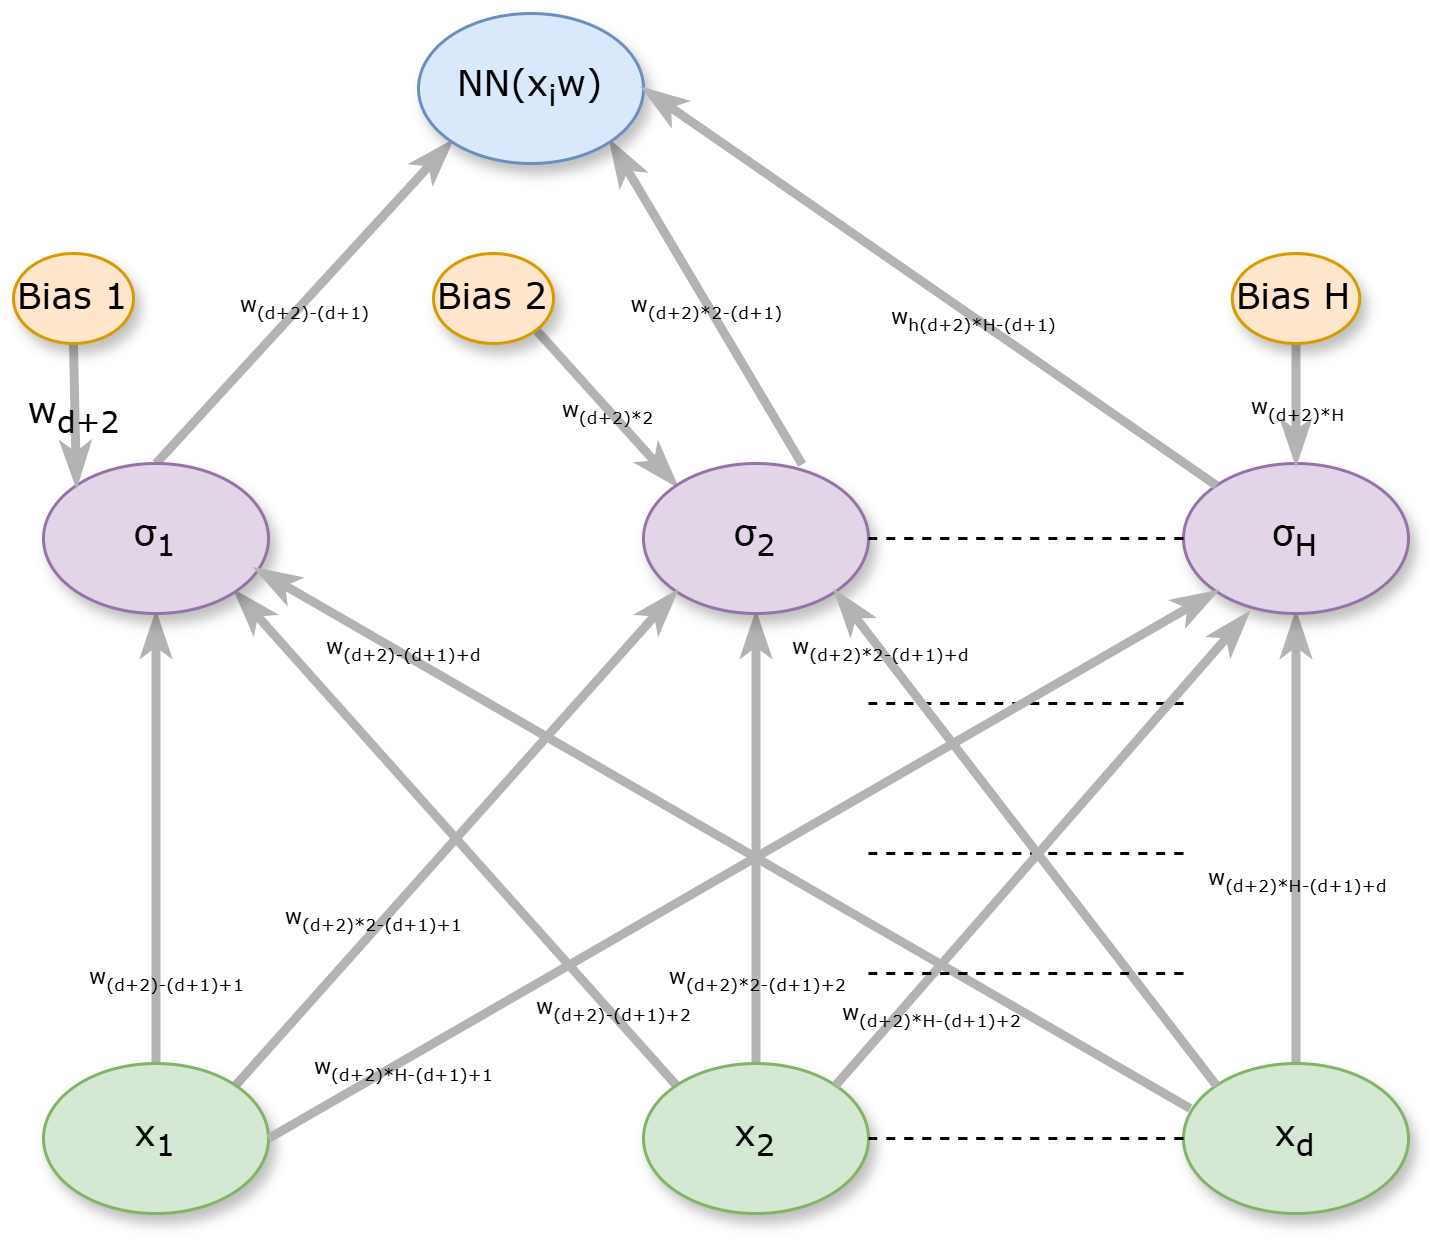
\includegraphics[scale=0.75]{flow2}
\par\end{centering}
\caption{The structure of the neural network incorporated in the current work.\label{fig:nnStructure}}

\end{figure}

Each chromosome in this genetic algorithm represents a possible set
of parameters for the artificial neural network and during optimization
the training error is minimized, as captured in equation \ref{eq:eq1}.
The main steps of this procedure have as follows:
\begin{enumerate}
\item \textbf{Initialization step}. 
\begin{enumerate}
\item \textbf{Define} as $N_{c}$ the number of chromosomes and as $N_{g}$
the maximum number of generations allowed before termination.
\item \textbf{Define} as $p_{s}$ the selection rate with $p_{s}\le$1.
\item \textbf{Define} as $p_{m}$ the mutation rate with $p_{m}\le$1.
\item \textbf{Initialize} randomly the chromosomes $g_{i},\ i=1,\ldots,N_{c}$.
\item \textbf{Set} $k=0$, the generation number.
\end{enumerate}
\item \textbf{Genetic operations step}.\label{enu:Genetic-operations-step.}
\begin{enumerate}
\item Fitness calculation. For every chromosome $c_{i},\ i=1,\ldots,N_{c}$
create the corresponding neural network $N\left(c_{i},x\right)$ and
set the corresponding fitness value with the following formula:
\[
f_{i}=\sum_{j=1}^{M}\left(N\left(c_{i},x_{j}\right)-y_{j}\right)^{2}
\]
\item Application of selection. The chromosomes and the corresponding fitness
values are sorted according to the fitness and the best $\left(1-p_{s}\right)\times N_{c}$
of them are copied intact to the next generation.\textbf{ }The rest
of the chromosomes are replaced by new chromosomes produced during
the crossover and the mutation procedure. 
\item Application of crossover. During this process, for every pair of constructed
chromosomes $\left(\tilde{z},\tilde{w}\right)$ two chromosomes $(z,w)$
are selected from the current population using tournament selection.
The construction of the new chromosomes is performed using the following:
\begin{eqnarray}
\tilde{z_{i}} & = & a_{i}z_{i}+\left(1-a_{i}\right)w_{i}\nonumber \\
\tilde{w_{i}} & = & a_{i}w_{i}+\left(1-a_{i}\right)z_{i}\label{eq:crossover_ali-1}
\end{eqnarray}
The values $a_{i}$ are random numbers with $a_{i}\in[-0.5,1.5]$
\citep{kaelo}. 
\item Application of mutation. For every element of each chromosomes a random
number $r\in[0,1]$ is drawn. This element is altered randomly when
$r\le p_{m}$.
\end{enumerate}
\item \textbf{Termination check}.
\begin{enumerate}
\item Set $k=k+1$
\item If $k\le N_{g}$ goto step \ref{enu:Genetic-operations-step.}
\end{enumerate}
\item \textbf{Finalization step}.
\begin{enumerate}
\item \textbf{Select} the chromosome $g^{*}$ with the lowest fitness value
from the population. 
\item \textbf{Define} the vectors $\overrightarrow{L},\overrightarrow{R}$
with the properties
\[
\begin{array}{ccc}
L_{i} & = & -F\left|g_{i}^{*}\right|\\
R_{i} & = & F\left|g_{i}^{*}\right|
\end{array},\ i=1,\ldots,n
\]
The parameter $F$ is a positive number with the property $F\ge1$.
\item The final outcome of the first phase is the vectors $\overrightarrow{L}$
and $\overrightarrow{R}$
\end{enumerate}
\end{enumerate}

\subsubsection{The second phase of the method}

In the second phase of the proposed methodology, an attempt is made
to estimate the optimal value intervals (bounds) of the artificial
neural network parameters. This phase initiates from the final outcome
of the previous phase, the vectors $\overrightarrow{L}$ and $\overrightarrow{R}$.
The estimation of the optimal value intervals is performed through
Grammatical Evolution, which utilizes the grammar shown in Figure
\ref{fig:BNF-grammar-of}.

\begin{figure}[H]
\begin{lyxcode}
S::=\textless expr\textgreater ~~~(0)~

\textless expr\textgreater ~::=~~(\textless xlist\textgreater ~,~\textless command\textgreater ,\textless command\textgreater )~~(0)~~~~~~~~~~~~~

~~~~~~~~~~~\textbar\textless expr\textgreater ,\textless expr\textgreater ~~~~~~~~~~~~~~~~~~~~(1)

\textless xlist\textgreater ::=x1~~~~(0)~~~~~~~~~~~~~~

~~~~~~~~~~~\textbar ~x2~(1)~~~~~~~~~~~~~~

~~~~~~~~~~~………~~~~~~~~~~~~~

~~~~~~~~~~~\textbar ~xn~(n-1)

\textless command\textgreater ~~::=~NOTHING~(0)~~~~~~~~~~~~~

~~~~~~~~~~~\textbar ~~~~~~~~SHRINK~~(1)

~~~~~~~~~~~\textbar ~~~~~~~~EXPAND~~(2)

~~~~~~~~~~~\textbar ~~~~~~~~SHRINK\_EXPAND~(3)

~~~~~~~~~~~\textbar ~~~~~~~~EXPAND\_SHRINK~(4)

~~~~~~~~~~~\textbar ~~~~~~~~SHRINK\_SHRINK~(5)

~~~~~~~~~~~\textbar ~~~~~~~~EXPAND\_EXPAND~(6)
\end{lyxcode}
\caption{BNF grammar used in the implemented work. The numbers in parentheses
denote the sequence number of the current production rule and they
are used during the Grammatical Evolution procedure in order to produce
valid programs. Symbols enclosed in \textless{} \textgreater{} are
considered non - terminal symbols of the grammar. The parameter n
denotes the number of parameters for the used neural network.\label{fig:BNF-grammar-of}}
\end{figure}
 This grammar proposes a series of commands that will be applied to
the bounds of the parameters of the neural network. These commands
are a series of expressions in the form (identifier,left\_command,right\_command).
The identifier represents the parameter where the command will be
applied, the left\_command indicates the command that will be executed
on the left bound of this parameter and the right\_command stands
for the command that will be applied on the right bound of the corresponding
parameter. These commands are:
\begin{enumerate}
\item NOTHING. Using this command does not change the limits of the corresponding
parameter. 
\item SHRINK. With this command, the corresponding bound is reduced by 50\%.
\item EXPAND. Activating this command results in the corresponding bound
being expanded by 50\%. 
\item SHRINK\_EXPAND. This command firstly reduces the corresponding bound
by 50\% and afterwards this bound is expanded by 50\%.
\item EXPAND\_SHRINK. This command firstly expands by 50\% the corresponding
bound and subsequently this bound is reduced by 50\%. 
\item SHRINK\_SHRINK. The execution of this command shrinks the corresponding
bound two times.
\item EXPAND\_EXPAND. This command expands the corresponding bound two times.
\end{enumerate}
As a full working example consider a neural network with $H=2$ processing
nodes and the consider also the dimension of the input patterns to
be $d=2$. The total number of variables for the neural network is
calculated as $n=(d+2)H=8$. Also, we consider that the initial values
of bounds are $\overrightarrow{L}=(-2,-4,-1,0,-4,-2,-1,-2)$ and $\overrightarrow{R}=(2,4,1,0,4,2,1,2)$.
Also, consider the chromosome

\textbf{
\[
g=\left[10,15,2,9,16,4,15,19,21\right]
\]
}The production steps for this example are shown in Table \ref{tab:Production-steps-for}. 

\begin{table}[H]
\caption{Production steps for the example considered here.\label{tab:Production-steps-for}}

\raggedright{}%
\begin{tabular}{|c|c|c|}
\hline 
{\footnotesize{}CHROMOSOME} & {\footnotesize{}ACTION} & {\footnotesize{}EXPRESSION}\tabularnewline
\hline 
\hline 
{\footnotesize{}10,15,2,9,16,4,15,19,21} & {\footnotesize{}10 mod 2=0} & {\footnotesize{}\textless expr\textgreater ,\textless expr\textgreater}\tabularnewline
\hline 
{\footnotesize{}15,2,9,16,4,15,19,21} & {\footnotesize{}15 mod 2 =1} & {\footnotesize{}(\textless xlist\textgreater ,\textless command\textgreater ,\textless command\textgreater ),\textless expr\textgreater}\tabularnewline
\hline 
{\footnotesize{}2,9,16,4,15,19,21} & {\footnotesize{}2\%8=2} & {\footnotesize{}(x3,\textless command\textgreater ,\textless command\textgreater ),\textless expr\textgreater}\tabularnewline
\hline 
{\footnotesize{}9,16,4,15,19,21} & {\footnotesize{}9\%7=2} & {\footnotesize{}(x3,EXPAND,\textless command\textgreater ),\textless expr\textgreater}\tabularnewline
\hline 
{\footnotesize{}16,4,15,19,21} & {\footnotesize{}16\%7=2} & {\footnotesize{}(x3,EXPAND,EXPAND),\textless expr\textgreater}\tabularnewline
\hline 
{\footnotesize{}4,15,19,21} & {\footnotesize{}4\%2=0} & {\footnotesize{}(x3,EXPAND,EXPAND),(\textless xlist\textgreater ,\textless command\textgreater ,\textless command\textgreater )}\tabularnewline
\hline 
{\footnotesize{}15,19,21} & {\footnotesize{}15\%8=7} & {\footnotesize{}(x3,EXPAND,EXPAND),(x8,\textless command\textgreater ,\textless command\textgreater )}\tabularnewline
\hline 
{\footnotesize{}19,21} & {\footnotesize{}19\%7=5} & {\footnotesize{}(x3,EXPAND,EXPAND),(x8,SHRINK\_EXPAND,\textless command\textgreater )}\tabularnewline
\hline 
{\footnotesize{}21} & {\footnotesize{}21\%7=0} & {\footnotesize{}(x3,EXPAND,EXPAND),(x8,SHRINK\_EXPAND,NOTHING)}\tabularnewline
\hline 
\end{tabular}
\end{table}
The final outcome of these steps is the expression 
\[
p=\left(x_{3},\mbox{EXPAND},\mbox{EXPAND}\right),\left(x8,\mbox{SHRINK\_EXPAND},\mbox{NOTHING}\right)
\]
After the application of the program $p$ to the vectors $\overrightarrow{L}$
and $\overrightarrow{R}$ the following vectors will be created: $\overrightarrow{L}=(-2,-4,-2,0,-4,-2,-1,-1),\overrightarrow{R}=(2,4,2,0,4,2,1,2).$
The analytical form for this example is the neural network defined
as:
\[
N\left(\overrightarrow{x},\overrightarrow{w}\right)=w_{1}\sigma\left(x_{1}w_{2}+x_{2}w_{3}+w_{4}\right)+w_{5}\sigma\left(x_{1}w_{6}+x_{2}w_{7}+w+w_{8}\right)
\]
For this specific example, the following applies to each variable
of the artificial neural network: 
\begin{enumerate}
\item $x_{1}\in[-2,2]$
\item $x_{2}\in[-4,4]$
\item $x_{3}\in[-2,2]$
\item $x_{4}\in[0,0]$. This variable can be considered as fixed to 0.0
\item $x_{5}\in[-4,4]$
\item $x_{6}\in[-2,2]$
\item $x_{7}\in[-1,1]$
\item $x_{8}\in[-1,2]$
\end{enumerate}
Furthermore, the method can significantly limit the value ranges of
the artificial neural network parameters or even set some of them
to zero. In this way, the method can indirectly construct the structure
of the neural network. A figure depicting the previously mentioned
example neural network is shown in Figure \ref{fig:exampleNN}.

\begin{figure}[H]
\begin{centering}
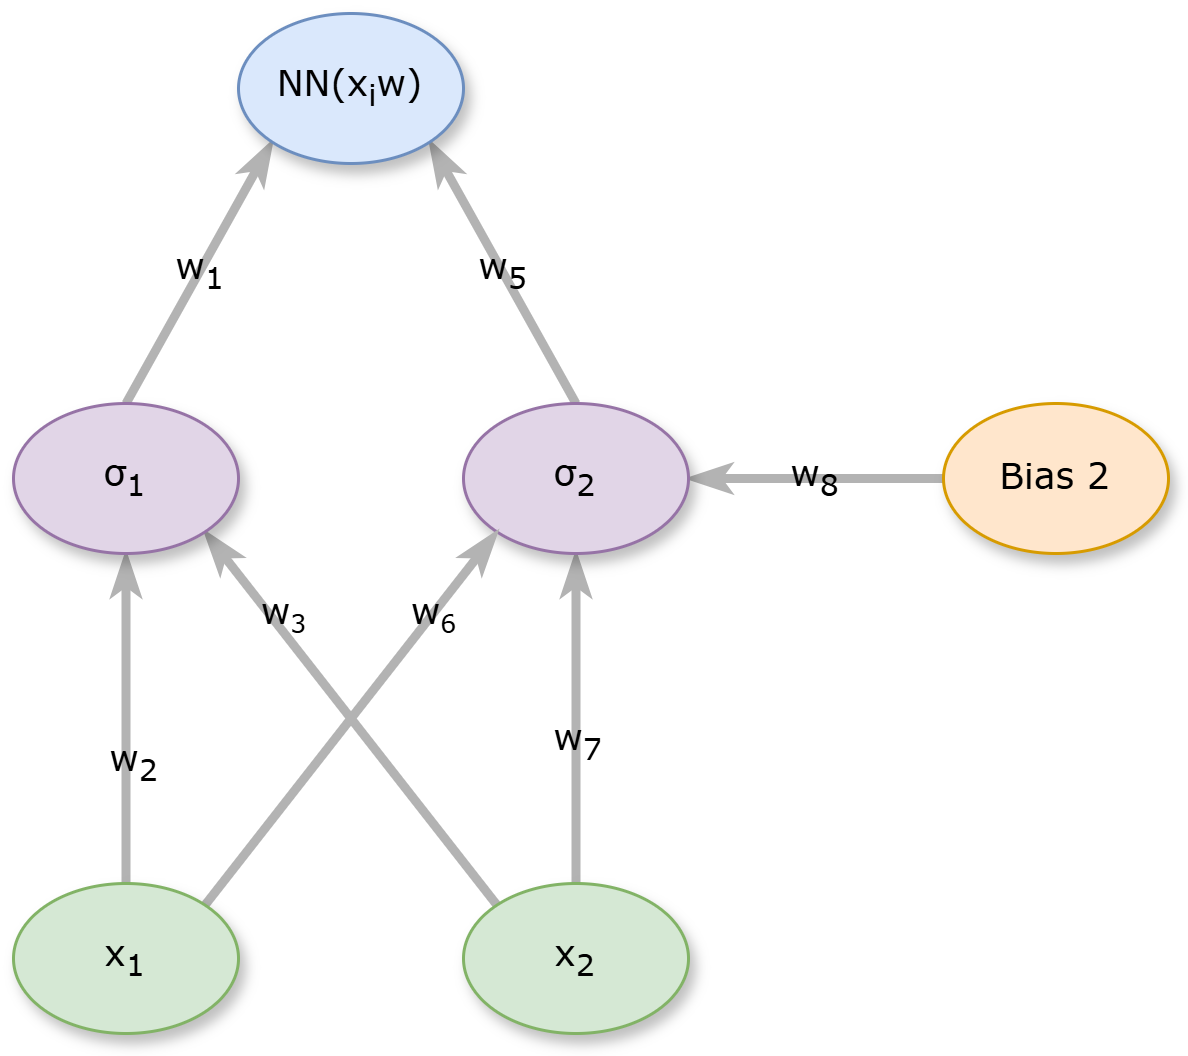
\includegraphics[scale=0.75]{flow1}
\par\end{centering}
\caption{A representation of the example neural network presented here.\label{fig:exampleNN}}

\end{figure}

The algorithm used in this phase is a variation of the genetic algorithm,
that incorporates the Grammatical Evolution procedure to create programs
that will be applied on the bounds of the neural network parameters.
The process used in this phase is a genetic algorithm, where the chromosomes
consist of value intervals for the parameters of the artificial neural
network. The fitness of each chromosome is considered as an interval,
and it is calculated through the process outlined in Algorithm \ref{alg:calcFitness}.

\begin{algorithm}[H]
\caption{Calculation of fitness value for every produced program $p$.\label{alg:calcFitness}}

\begin{enumerate}
\item \textbf{Set} as $N_{s}$ the number of random samples that will be
used.
\item \textbf{Set} $f_{l}=\infty$
\item \textbf{Set} $f_{u}=-\infty$
\item \textbf{Apply} the program $p$ to the bounds of the neural network
to produce the new bounds $\overrightarrow{L_{p}},\overrightarrow{R_{p}}$.
\item \textbf{For} $i=1,\ldots,N_{s}$ \textbf{do}
\begin{enumerate}
\item \textbf{Create} randomly the set $w_{p}\in$$\left[\vec{L_{p}},\overrightarrow{R_{p}}\right]$
as a new set of parameters for the neural network.
\item \textbf{Calculate} the training error $E_{w}=\sum_{k=1}^{M}\left(N\left(\overrightarrow{x}_{k},\overrightarrow{w_{p}}\right)-y_{k}\right)^{2}$
\item \textbf{If} $E_{w}\le f_{l}$ then $f_{l}=E_{w}$
\item \textbf{If} $E_{w}\ge f_{u}$ then $f_{u}=E_{w}$
\end{enumerate}
\item \textbf{End For}
\item \textbf{Return} as fitness value the interval $\left[f_{l},f_{u}\right]$.
\end{enumerate}
\end{algorithm}

The steps of the proposed algorithm for the second phase are the following:
\begin{enumerate}
\item \textbf{Initialization Step}.
\begin{enumerate}
\item \textbf{Define} as $N_{c}$ the population size and denote as $N_{g}$
the maximum number of generations allowed.
\item \textbf{Define} as $p_{s}$ the selection rate with $p_{s}\le$1.
\item \textbf{Define} as $p_{m}$ the mutation rate with $p_{m}\le$1.
\item \textbf{Define} as $p_{l}$ the used local search rate with $p_{l}\le$1
\item \textbf{Set} as $N_{s}$ the number of samples that will be used during
the fitness calculation.
\item \textbf{Set} as $N_{L}$ the number of chromosomes that will participate
in the local search procedure.
\item \textbf{Initialize }randomly the chromosomes $g_{i},\ i=1,\ldots,N_{c}$.
Each chromosome is a set of randomly selected positive integers.
\item \textbf{Set }$k=0$, the generation number.
\end{enumerate}
\item \textbf{Fitness calculation step}.\label{enu:Fitness-calculation-step.}
\begin{enumerate}
\item \textbf{For} every chromosome $g_{i},\ i=1,\ldots,N_{c}$ \textbf{do}
\begin{enumerate}
\item \textbf{Create} the corresponding program $p_{i}$ using the Grammatical
Evolution procedure and the associated BNF grammar outlined in Figure
\ref{fig:BNF-grammar-of}.
\item \textbf{Calculate} the fitness value $f_{i}$ for program $p_{i}$
using the algorithm shown in Algorithm \ref{alg:calcFitness}.
\end{enumerate}
\item \textbf{End For}
\end{enumerate}
\item \textbf{Genetic operations step}.
\begin{enumerate}
\item Application of selection. During the selection procedure the chromosome
are firstly sorted according to their fitness values. The comparison
of any pair of fitness values $f_{a}=\left[a_{1},a_{2}\right]$ and
$f_{b}=\left[b_{1},b_{2}\right]$ is performed using the following
operator:
\begin{eqnarray}
L^{*}\left(f_{a},f_{b}\right) & = & \begin{cases}
\mbox{TRUE}, & a_{1}<b_{1},\mbox{OR\ \ensuremath{\left(a_{1}=b_{1}\ \mbox{AND}\ a_{2}<b_{2}\right)}}\\
\mbox{FALSE}, & \mbox{\mbox{OTHERWISE}}
\end{cases}\label{eq:eql}
\end{eqnarray}
The $\left(1-p_{s}\right)\times N_{c}$ chromosomes with the lowest
fitness values according to the previous operator are copied intact
to the next generation. The remaining of them are replaced by chromosomes
produced through crossover and mutation.
\item Application of crossover. During this procedure, for every pair of
produced chromosomes $\left(\tilde{z},\tilde{w}\right)$ two chromosomes
$(z,w)$ are selected from the current population with the assistance
of tournament selection. The new chromosomes are constructed using
one - point crossover, that is graphically outlined in Figure \ref{fig:onePoint}.
\item Application of mutation. Every element of each chromosome is altered
with probability $p_{m}$. During this procedure a random integer
value is selected and it replaces the chosen element of the under
processing chromosome.
\end{enumerate}
\item \textbf{Local search step}.
\begin{enumerate}
\item \textbf{For} each chromosome $g_{i},\ i=1,\ldots,N_{c}$ \textbf{do}
\begin{enumerate}
\item \textbf{Draw} a random number $r\in[0,1]$
\item \textbf{If} $r\le p_{l}$ then alter randomly chromosome $g_{i}$
with the procedure described in Algorithm \ref{alg:localSearch}.
\end{enumerate}
\item \textbf{End for}
\end{enumerate}
\item \textbf{Termination check step}.
\begin{enumerate}
\item \textbf{Set} $k=k+1$
\item \textbf{If} $k\ge N_{g}$ terminate else goto step \ref{enu:Fitness-calculation-step.}.
\item \textbf{Report} $g^{*}$ as the final outcome of this algorithm having
the lowest fitness value among the chromosomes of the population.
The application of this chromosome to the bounds of the neural network
will produce the set of bounds $\overrightarrow{L^{*}}$ and $\overrightarrow{R^{*}}$.
\end{enumerate}
%
\end{enumerate}
\begin{figure}[H]
\begin{centering}
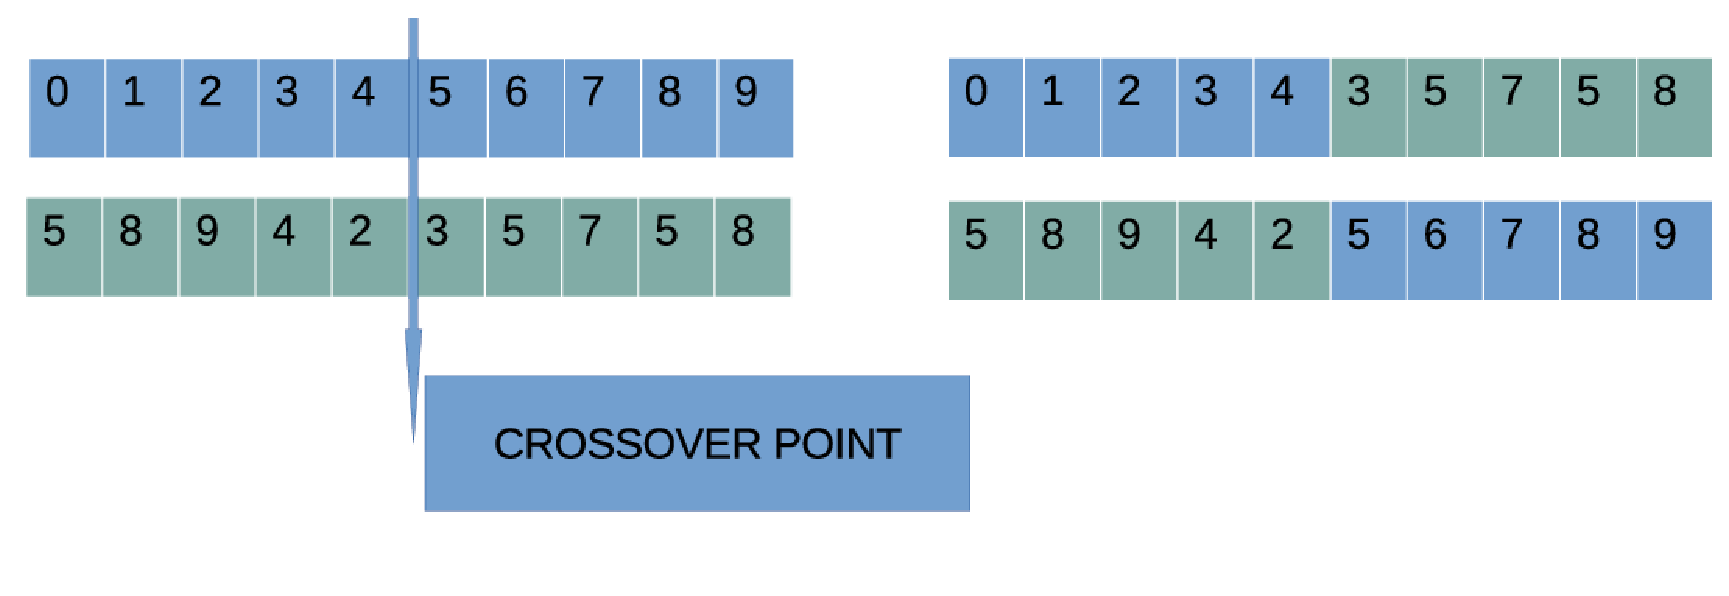
\includegraphics[scale=0.5]{onepoint_crossover}
\par\end{centering}
\caption{An example of one - point crossover mechanism, used in the Grammatical
Evolution procedure.\label{fig:onePoint}}

\end{figure}
\begin{algorithm}[H]
\caption{Local search procedure applied on a chromosome $g$.\label{alg:localSearch}}

\begin{enumerate}
\item \textbf{Set} as $f_{g}$ the corresponding fitness value of chromosome
$g$.
\item \textbf{Create} randomly the set $C=\left\{ x_{1},x_{2},\ldots,x_{N_{l}}\right\} $
of $N_{l}$ chromosomes from the current population.
\item \textbf{For} $i=1,\ldots,N_{cr}$ \textbf{do}
\begin{enumerate}
\item \textbf{Execute }the one - point crossover using chromosomes $g$
and $x_{i}$. The one - point crossover will create two chromosomes:
$g_{1}$ and $g_{2}$ and the related fitness values are $f_{g_{1}}$
and $f_{g_{2}}$.
\item \textbf{If} $f_{g_{1}}\le f_{g}$ \textbf{then} $g=g_{1}$ 
\item \textbf{else if} $f_{g_{2}}\le f_{g}$ \textbf{then} $g=g_{2}$
\item \textbf{End if}
\end{enumerate}
\item \textbf{End For}
\end{enumerate}
\end{algorithm}

The purpose of this phase of the algorithm is to identify the most
promising range of values for the parameters of the artificial neural
network through the application of partitioning rules. Furthermore,
the above procedure will significantly reduce the local minima contained
in the error function, since the initial search space will be significantly
limited to only those regions that may contain the global minimum
or approximations thereof. 

\subsubsection{The final phase of the method}

During the last phase of the proposed method, the bounds $\overrightarrow{L^{*}}$
and $\overrightarrow{R^{*}}$ produced by the previous phase are evaluated
using a modified genetic algorithm, used to train the artificial neural
network.
\begin{enumerate}
\item \textbf{Initialization step}.
\begin{enumerate}
\item \textbf{Set} as $N_{c}$ the number of chromosomes and as $N_{g}$
the maximum number of generations.
\item \textbf{Set} as $p_{s}$ the selection rate and as $p_{m}$ the mutation
rate.
\item \textbf{Initialize} randomly each chromosome $g_{i},\ i=1,\ldots,N_{c}$
inside the bounds $\overrightarrow{L^{*}}$ and $\overrightarrow{R^{*}}$
of the previous procedure. 
\item \textbf{Set} $k=0$ the generation number.
\end{enumerate}
\item \textbf{Fitness Calculation step}. For every chromosome $g_{i},\ i=1,\ldots,N_{c}$
create the corresponding neural network $N\left(g_{i},x\right)$ and
set the corresponding fitness value with the following formula:
\[
f_{i}=\sum_{j=1}^{M}\left(N\left(g_{i},x_{j}\right)-y_{j}\right)^{2}
\]
\label{enu:ff2}
\item \textbf{Application of genetic operations}.
\begin{enumerate}
\item Application of selection. The chromosomes are sorted according to
their fitness. The best $\left(1-p_{s}\right)\times N_{c}$ of them
will be copied to the next generation, while the remaining ones will
be substituted by chromosomes produced during crossover and mutation.
\item Application of crossover. For each pair of produced chromosomes $(\widetilde{z},\widetilde{w})$
two chromosomes $z$ and $w$ from the current population will be
selected through tournament selection. The new chromosomes will be
formed with a process similar with this of the crossover procedure
of the first stage of the current work. 
\item Application of mutation. Every element of each chromosome is altered
with probability $p_{m}$. 
\end{enumerate}
\item \textbf{Termination check step}.
\begin{enumerate}
\item \textbf{Set} $k=k+1$
\item \textbf{If} $k\le N_{G}$ then goto step \ref{enu:ff2}.
\end{enumerate}
\item \textbf{Local search step}.
\begin{enumerate}
\item \textbf{Obtain} the best chromosome $g^{*}$ from the population and
form the corresponding neural network $N\left(g^{*},x\right)$ 
\item \textbf{Minimize} the associated training error 
\[
f^{*}=\sum_{j=1}^{M}\left(N\left(g_{i}^{*},x_{j}\right)-y_{j}\right)^{2}
\]
using a local search procedure. In the proposed method the BFGS variant
of Powell \citep{powell} was used.
\end{enumerate}
\end{enumerate}

\section{Results\label{sec:Results}}

The new training procedure for the construction of weights of neural
networks was tested on a wide series of classification and regression
datasets, found in the recent literature and in the following websites:
\begin{enumerate}
\item The UCI website, \url{https://archive.ics.uci.edu/}(accessed on 24
November 2024)\citep{uci}
\item The Keel website, \url{https://sci2s.ugr.es/keel/datasets.php}(accessed
on 24 November 2024)\citep{Keel}.
\item The Statlib URL \url{ftp://lib.stat.cmu.edu/datasets/index.html }(accessed
on 24 November 2024). 
\end{enumerate}

\subsection{Datasets }

The following classification datasets were incorporated in the conducted
experiments:
\begin{enumerate}
\item \textbf{Alcohol}. This dataset is related to experiments on alcohol
consumption \citep{alcohol}. 
\item \textbf{Australian}, related to economic risk in bank transactions
\citep{australian}.
\item \textbf{Bands}, related to printing problems \citep{bands}, with
two distinct classes.
\item \textbf{Cleveland}, a medical dataset studied in many research papers
\citep{cleveland1,cleveland2}. 
\item \textbf{Circular} dataset, which is an artificial dataset.
\item \textbf{Dermatology}, a medical dataset related to dermatology problems
\citep{dermatology} with 6 classes.
\item \textbf{Ecoli}, that is related to issues about proteins \citep{ecoli}.
\item \textbf{Haberman}, a medical dataset used in the detection of breast
cancer. 
\item \textbf{Hayes-roth} dataset \citep{hayes-roth}, a dataset with 3
classes.
\item \textbf{Heart}, a medical dataset about heart diseases \citep{heart}
with two classes.
\item \textbf{HeartAttack}, a medical dataset related to the presence of
heart diseases, with two classes.
\item \textbf{Hepatitis}, a dataset used for to detect the presence of hepatitis. 
\item \textbf{Housevotes}, that uses data from the Congressional voting
in USA \citep{housevotes}.
\item \textbf{Ionosphere}, that used data from various measurements in the
ionosphere \citep{ion1,ion2}.
\item \textbf{Liverdisorder}, which is a medical dataset \citep{liver,liver1}
with two classes.
\item \textbf{Lymography} \citep{lymography}, which is a dataset with four
distinct classes.
\item \textbf{Magic}, this dataset contains data from simulation regarding
gamma particles \citep{magic}.
\item \textbf{Mammographic}, a medical dataset used for the detection of
 breast cancer \citep{mammographic}.
\item \textbf{Page Blocks }dataset \citep{pageblocks}, which is incorporated
for the detection of page layout in documents.
\item \textbf{Parkinsons}, a dataset used to detect the presence of Parkinson's
disease \citep{parkinsons1,parkinsons2}.
\item \textbf{Pima}, a medical dataset that used to detect the presence
of diabetes\citep{pima}.
\item \textbf{Phoneme}, where the purpose of this dataset is to distinguish
between nasal and oral sounds.
\item \textbf{Popfailures}, a dataset related to climate measurements \citep{popfailures}.
\item \textbf{Regions2}, used detect issues in the liver from various liver
biopsy images \citep{regions2}.
\item \textbf{Ring}, a dataset related to some multivariate normal distributions. 
\item \textbf{Saheart}, used to detect the presence of some heart diseases.\citep{saheart}.
\item \textbf{Segment} dataset \citep{segment}, which is used for image
processing .
\item \textbf{Statheart}, a medical dataset about heart diseases.
\item \textbf{Spambase}, a dataset used for the detection of spam emails. 
\item \textbf{Spiral}, which is an artificial dataset.
\item \textbf{Student}, a dataset related to some experiments in schools
\citep{student}.
\item \textbf{Tae}, this dataset is related to evaluations of teaching performance.
\item \textbf{Transfusion}, which is a medical dataset \citep{transfusion}.
\item \textbf{Wdbc}, a medical dataset related to the detection of breast
cancer \citep{wdbc1,wdbc2}.
\item \textbf{Wine}, a dataset related to the quality of wines \citep{wine1,wine2}.
\item \textbf{EEG} dataset, which is a medical dataset related to EEG measurements\citep{eeg1,eeg2}.
From the original dataset the following cases were obtained: Z\_F\_S,
ZO\_NF\_S, Z\_O\_N\_F\_S and ZONF\_S.
\item \textbf{Zoo}, that used to predict the class of some animals \citep{zoo}
.
\end{enumerate}
Also the following regression datasets were used in the conducted
experiments:
\begin{enumerate}
\item \textbf{Abalone}, a dataset regarding the prediction of the age of
abalones \citep{abalone}.
\item \textbf{Airfoil}, a dataset derived from NASA \citep{airfoil} with
5 features.
\item \textbf{Auto}, a dataset used for the prediction of fuel consumption
in cars.
\item \textbf{BK}, related to basketball games. The dataset has 4 features.
\item \textbf{BL}, a dataset used in some electricity experiments and it
contains 7 features.
\item \textbf{Baseball}, a dataset with 16 features used for the estimation
of the income of baseball players.
\item \textbf{Concrete}, a dataset with 8 features and it was used in civil
engineering \citep{concrete}.
\item \textbf{DEE}, a dataset with 6 features, used in the prediction of
electricity prices.
\item \textbf{EU}, a dataset originated in the STATLIB website.
\item \textbf{FA}, that contains related to body fat.
\item \textbf{Friedman}, a synthetic dataset used in various benchmarks
\citep{friedman}.
\item \textbf{FY, }this dataset used to measure the longevity of fruit flies. 
\item \textbf{HO}, a dataset founded in the STATLIB repository with 13 features.
\item \textbf{Housing}, used to predict the price of houses \citep{housing}.
\item \textbf{Laser}, which is a dataset with 4 features and it has been
used in various laser experiments.
\item \textbf{LW}, a dataset with 9 features used to measure the weight
of babes.
\item \textbf{Mortgage}, an economic dataset with 15 features.
\item \textbf{Plastic}, a dataset related to the detection of pressure on
plastics.
\item \textbf{PL}, a dataset with 2 features founded in the STATLIB repository.
\item \textbf{RealEstate, }a dataset found in the STATLIB website with 5
features.
\item \textbf{Quake}, a dataset used in earthquake measurements with 3 features.
\item \textbf{SN}, a dataset that provides experimental measurements related
to trellising and pruning, with 11 features.
\item \textbf{Stock}, a dataset with 9 features for the prediction of the
prices of various stocks.
\item \textbf{Treasury}, an economic dataset with 15 features.
\item \textbf{TZ}, derived from the STATLIB website and it has 60 features.
\item \textbf{VE} dataset, derived from the STALIB repository.
\end{enumerate}

\subsection{Experimental results}

The algorithm used in the current work was coded in ANSI C++. All
the runs were performed 30 times using different seeds for the random
generator each time. The validation of the experiments was performed
using the 10 - fold validation technique. The experiments were carried
out on an AMD Ryzen 5950X with 128GB of RAM. The used operating system
was Debian Linux. In Table \ref{tab:settings} the values used in
all experimental parameters are listed.\textbf{ }
\begin{table}[H]
\caption{The values used for all experimental parameters of the proposed method.\label{tab:settings}}

\centering{}%
\begin{tabular}{|c|c|c|}
\hline 
PARAMETER & MEANING & VALUE\tabularnewline
\hline 
\hline 
$N_{g}$ & Number of generations allowed & 200\tabularnewline
\hline 
$N_{c}$ & Number of chromosomes & 500\tabularnewline
\hline 
$N_{s}$ & Number of samples & 50\tabularnewline
\hline 
$N_{l}$ & Number of chromosome used in local search & 20\tabularnewline
\hline 
$p_{s}$ & Selection rate & 0.1\tabularnewline
\hline 
$p_{m}$ & Mutation rate & 0.05\tabularnewline
\hline 
$p_{l}$ & Local search rate & 0.001\tabularnewline
\hline 
$H$ & Number of processing nodes & 10\tabularnewline
\hline 
\end{tabular}
\end{table}
\textbf{ }The table \ref{tab:expClass} outlines the experimental
results for the classification datasets and in Table \ref{tab:expRegression}
the experimental results for the regression datasets are listed.\textbf{
}The classification error is defined as:
\begin{equation}
E_{C}\left(M(x)\right)=100\times\frac{\sum_{i=1}^{N}\left(\mbox{class}\left(M\left(x_{i}\right)\right)-y_{i}\right)}{N}
\end{equation}
where $M(x)$ denotes the underlying machine learning model and set
$T$ stands for the train dataset.\textbf{ }Also, the regression error
is defined as: 
\begin{equation}
E_{R}\left(M(x)\right)=\frac{\sum_{i=1}^{N}\left(M\left(x_{i}\right)-y_{i}\right)^{2}}{N}
\end{equation}
The following applies to these tables:
\begin{enumerate}
\item The column DATASET represents the used dataset.
\item The column ADAM denotes the application of the ADAM optimizer to a
neural network with $H=10$ processing nodes.
\item The column BFGS stands for the application of the BFGS variant of
Powell to a neural network with $H=10$ processing nodes.
\item The column GENETIC stands for the usage of a genetic algorithm on
a neural network with $H=10$ processing nodes. The values for the
parameters of this genetic algorithm are shown in Table \ref{tab:settings}.
\item The column NEAT defines the application of the NEAT method (NeuroEvolution
of Augmenting Topologies ) \citep{neat} as implemented in EvolutionNet
package freely available from \url{https://github.com/BiagioFesta/EvolutionNet}.
The number of used generations is the same as in the GENETIC algorithm. 
\item The column RBF stands for the usage of a Radial Basis Function (RBF)
network \citep{rbf1,rbf2} with $H=10$ processing nodes.
\item The column GNN stands for the incorporation of the proposed method
to a neural network with $H=10$ processing nodes with parameter settings
outlined in Table \ref{tab:settings}.
\item The row denoted as AVERAGE represents the average classification or
regression error for all datasets.
\end{enumerate}
\begin{table}[H]
\caption{Experimental results for the classification datasets. Numbers in cells
denote the average classification error as calculated on the corresponding
test set.\label{tab:expClass}}

\centering{}%
\begin{tabular}{|c|c|c|c|c|c|c|}
\hline 
DATASET & ADAM & BFGS & GENETIC & NEAT & RBF & GNN\tabularnewline
\hline 
\hline 
ALCOHOL & 57.78\% & 41.50\% & 39.57\% & 66.80\% & 49.32\% & 16.63\%\tabularnewline
\hline 
AUSTRALIAN & 35.65\% & 38.13\% & 32.21\% & 31.98\% & 34.89\% & 14.69\%\tabularnewline
\hline 
BALANCE & 12.27\% & 8.64\% & 8.97\% & 23.14\% & 33.53\% & 7.98\%\tabularnewline
\hline 
BANDS & 36.92\% & 36.67\% & 34.92\% & 34.30\% & 37.17\% & 34.38\%\tabularnewline
\hline 
CLEVELAND & 67.55\% & 77.55\% & 51.60\% & 53.44\% & 67.10\% & 44.89\%\tabularnewline
\hline 
CIRCULAR & 19.95\% & 6.08\% & 5.99\% & 35.18\% & 5.98\% & 4.68\%\tabularnewline
\hline 
DERMATOLOGY & 26.14\% & 52.92\% & 30.58\% & 32.43\% & 62.34\% & 11.79\%\tabularnewline
\hline 
ECOLI & 64.43\% & 69.52\% & 54.67\% & 43.44\% & 59.48\% & 51.42\%\tabularnewline
\hline 
HABERMAN & 29.00\% & 29.34\% & 28.66\% & 24.04\% & 25.10\% & 27.01\%\tabularnewline
\hline 
HAYES-ROTH & 59.70\% & 37.33\% & 56.18\% & 50.15\% & 64.36\% & 34.99\%\tabularnewline
\hline 
HEART & 38.53\% & 39.44\% & 28.34\% & 39.27\% & 31.20\% & 14.83\%\tabularnewline
\hline 
HEARTATTACK & 45.55\% & 46.67\% & 29.03\% & 32.34\% & 29.00\% & 19.23\%\tabularnewline
\hline 
HEPATITIS & 68.13\% & 72.47\% & 62.12\% & 67.04\% & 64.63\% & 56.67\%\tabularnewline
\hline 
HOUSEVOTES & 7.48\% & 7.13\% & 6.62\% & 10.89\% & 6.13\% & 6.23\%\tabularnewline
\hline 
IONOSPHERE & 16.64\% & 15.29\% & 15.14\% & 19.67\% & 16.22\% & 15.71\%\tabularnewline
\hline 
LIVERDISORDER & 41.53\% & 42.59\% & 31.11\% & 30.67\% & 30.84\% & 31.89\%\tabularnewline
\hline 
LYMOGRAPHY & 39.79\% & 35.43\% & 28.42\% & 33.70\% & 25.50\% & 19.26\%\tabularnewline
\hline 
MAGIC & 40.55\% & 17.30\% & 21.75\% & 24.85\% & 21.28\% & 15.67\%\tabularnewline
\hline 
MAMMOGRAPHIC & 46.25\% & 17.24\% & 19.88\% & 22.85\% & 21.38\% & 16.33\%\tabularnewline
\hline 
PARKINSONS & 24.06\% & 27.58\% & 18.05\% & 18.56\% & 17.41\% & 11.53\%\tabularnewline
\hline 
PAGE BLOCKS & 34.27\% & 8.49\% & 6.84\% & 10.22\% & 10.09\% & 7.66\%\tabularnewline
\hline 
PHONEME & 29.43\% & 15.58\% & 15.55\% & 22.34\% & 23.32\% & 16.59\%\tabularnewline
\hline 
PIMA & 34.85\% & 35.59\% & 32.19\% & 34.51\% & 25.78\% & 25.81\%\tabularnewline
\hline 
POPFAILURES & 5.18\% & 5.24\% & 5.94\% & 7.05\% & 7.04\% & 5.25\%\tabularnewline
\hline 
REGIONS2 & 29.85\% & 36.28\% & 29.39\% & 33.23\% & 38.29\% & 29.24\%\tabularnewline
\hline 
RING & 28.80\% & 29.44\% & 28.80\% & 30.85\% & 21.67\% & 21.68\%\tabularnewline
\hline 
SAHEART & 34.04\% & 37.48\% & 34.86\% & 34.51\% & 32.19\% & 29.92\%\tabularnewline
\hline 
SEGMENT & 49.75\% & 68.97\% & 57.72\% & 66.72\% & 59.68\% & 31.21\%\tabularnewline
\hline 
SONAR & 30.33\% & 25.85\% & 22.40\% & 34.10\% & 27.90\% & 22.80\%\tabularnewline
\hline 
SPAMBASE & 48.05\% & 18.16\% & 6.37\% & 35.77\% & 29.35\% & 6.17\%\tabularnewline
\hline 
SPIRAL & 47.67\% & 47.99\% & 48.66\% & 48.66\% & 44.87\% & 41.97\%\tabularnewline
\hline 
STATHEART & 44.04\% & 39.65\% & 27.25\% & 44.36\% & 31.36\% & 18.20\%\tabularnewline
\hline 
STUDENT & 5.13\% & 7.14\% & 5.61\% & 10.20\% & 5.49\% & 4.98\%\tabularnewline
\hline 
TAE & 60.20\% & 51.58\% & 49.84\% & 60.67\% & 60.02\% & 48.89\%\tabularnewline
\hline 
TRANSFUSION & 25.68\% & 25.84\% & 24.87\% & 24.87\% & 26.41\% & 23.34\%\tabularnewline
\hline 
WDBC & 35.35\% & 29.91\% & 8.56\% & 12.88\% & 7.27\% & 3.70\%\tabularnewline
\hline 
WINE & 29.40\% & 59.71\% & 19.20\% & 25.43\% & 31.41\% & 9.14\%\tabularnewline
\hline 
Z\_F\_S & 47.81\% & 39.37\% & 10.73\% & 38.41\% & 13.16\% & 8.35\%\tabularnewline
\hline 
Z\_O\_N\_F\_S & 78.79\% & 65.67\% & 64.81\% & 77.08\% & 48.70\% & 60.83\%\tabularnewline
\hline 
ZO\_NF\_S & 47.43\% & 43.04\% & 21.54\% & 43.75\% & 9.02\% & 6.29\%\tabularnewline
\hline 
ZONF\_S & 11.99\% & 15.62\% & 4.36\% & 5.44\% & 4.03\% & 2.77\%\tabularnewline
\hline 
ZOO & 14.13\% & 10.70\% & 9.50\% & 20.27\% & 21.93\% & 6.03\%\tabularnewline
\hline 
\textbf{AVERAGE} & \textbf{36.91\%} & \textbf{34.19\%} & \textbf{27.11\%} & \textbf{33.72\%} & \textbf{30.52\%} & \textbf{21.11\%}\tabularnewline
\hline 
\end{tabular}
\end{table}
\begin{table}[H]
\caption{Experimental results for the series of regression datasets. The numbers
in cells correspond to the average regression error of each test set.\label{tab:expRegression}}

\centering{}%
\begin{tabular}{|c|c|c|c|c|c|c|}
\hline 
DATASET & ADAM & BFGS & GENETIC & NEAT & RBF & GNN\tabularnewline
\hline 
\hline 
ABALONE & 4.30 & 5.69 & 7.17 & 9.88 & 7.37 & 4.32\tabularnewline
\hline 
AIRFOIL & 0.005 & 0.003 & 0.003 & 0.067 & 0.27 & 0.001\tabularnewline
\hline 
AUTO & 70.84 & 60.97 & 12.18 & 56.06 & 17.87 & 8.69\tabularnewline
\hline 
BK & 0.0252 & 0.28 & 0.027 & 0.15 & 0.02 & 0.039\tabularnewline
\hline 
BL & 0.622 & 2.55 & 5.74 & 0.05 & 0.013 & 0.013\tabularnewline
\hline 
BASEBALL & 77.90 & 119.63 & 103.60 & 100.39 & 93.02 & 47.25\tabularnewline
\hline 
CONCRETE & 0.078 & 0.066 & 0.0099 & 0.081 & 0.011 & 0.004\tabularnewline
\hline 
DEE & 0.63 & 2.36 & 1.013 & 1.51 & 0.17 & 0.212\tabularnewline
\hline 
EU & 604.253 & 608.99 & 252.97 & 397.27 & 235.14 & 148.76\tabularnewline
\hline 
FA & 0.048 & 0.426 & 0.025 & 0.19 & 0.015 & 0.097\tabularnewline
\hline 
FRIEDMAN & 22.896 & 1.263 & 1.249 & 19.35 & 7.23 & 1.573\tabularnewline
\hline 
FY & 0.038 & 0.22 & 0.65 & 0.08 & 0.04 & 0.121\tabularnewline
\hline 
HO & 0.035 & 0.62 & 2.78 & 0.17 & 0.03 & 0.05\tabularnewline
\hline 
HOUSING & 80.998 & 97.38 & 43.26 & 56.49 & 57.68 & 14.79\tabularnewline
\hline 
LASER & 0.03 & 0.015 & 0.59 & 0.084 & 0.03 & 0.0029\tabularnewline
\hline 
LW & 0.028 & 2.98 & 1.90 & 0.17 & 0.03 & 0.313\tabularnewline
\hline 
MORTGAGE & 9.24 & 8.23 & 2.41 & 14.11 & 1.45 & 0.0222\tabularnewline
\hline 
PLASTIC & 11.713 & 20.323 & 2.791 & 20.77 & 8.62 & 2.186\tabularnewline
\hline 
PY & 0.321 & 0.578 & 0.56 & 0.075 & 0.012 & 0.111\tabularnewline
\hline 
PL & 0.117 & 0.29 & 0.28 & 0.098 & 2.12 & 0.0205\tabularnewline
\hline 
REALESTATE & 186.778 & 170.28 & 81.19 & 155.46 & 76.50 & 70.928\tabularnewline
\hline 
QUAKE & 0.07 & 0.42 & 0.04 & 0.298 & 0.07 & 0.04\tabularnewline
\hline 
SN & 0.026 & 0.40 & 2.95 & 0.174 & 0.027 & 0.025\tabularnewline
\hline 
STOCK & 180.893 & 302.43 & 3.881 & 215.82 & 12.23 & 2.986\tabularnewline
\hline 
TREASURY & 11.16 & 9.91 & 2.929 & 15.52 & 2.02 & 0.0633\tabularnewline
\hline 
TZ & 0.07 & 3.27 & 5.38 & 0.098 & 0.036 & 0.652\tabularnewline
\hline 
VE & 0.359 & 1.92 & 2.43 & 0.045 & 0.024 & 0.0493\tabularnewline
\hline 
\textbf{AVERAGE} & \textbf{46.795} & \textbf{52.648} & \textbf{19.926} & \textbf{39.42} & \textbf{19.34} & \textbf{11.234}\tabularnewline
\hline 
\end{tabular}
\end{table}
 The statistical analysis of Table \ref{tab:expClass} highlights
interesting patterns regarding model performance and the nature of
the datasets. The GNN model achieves the lowest average error rate
(21.11\%), making it the overall best-performing model. This suggests
that it is particularly effective across the dataset collection. In
contrast, NEAT, despite an average error rate of 33.72\%, excels in
specific datasets such as Z\_O\_N\_F\_S, where it performs almost
equivalently to GNN. The analysis reveals significant variations in
error rates across datasets, indicating differing levels of complexity
and challenges faced by the models. For instance, datasets like Z\_O\_N\_F\_S,
where errors are low for all models, are likely characterized by well-defined
patterns and minimal class overlap. On the other hand, datasets such
as SPAMBASE and MAGIC appear more complex, with high error rates across
many models. In SPAMBASE, GNN's performance (6.17\%) is remarkable,
indicating its superior capability in handling such data compared
to other models. ADAM, with an average error rate of 36.91\%, demonstrates
consistent but not top-tier performance. This model seems reliable
for medium-complexity datasets, such as BANDS and AUSTRALIAN, where
it achieves comparable or better results than other models. However,
it underperforms in high-dimensional datasets, such as SEGMENT, where
BFGS significantly outperforms it. BFGS exhibits strong performance
in problems like DERMATOLOGY, likely due to its adaptability to data
with well-defined boundaries. The GENETIC model shows intriguing behavior,
excelling in datasets such as ZONF\_S and RING, but lagging in higher
complexity problems like HEPATITIS. This indicates potential limitations
in processing high-dimensional or noisy data. Conversely, RBF appears
particularly sensitive to dataset-specific characteristics, performing
well in certain datasets like BALANCE but falling short in problems
such as SPIRAL and HOUSEVOTES. The comparison between models underscores
the necessity of tailored model selection for each dataset. For instance,
GNN would be the preferred choice for problems demanding the lowest
possible error, while ADAM would be ideal for cases where stability
and generalization are more critical. NEAT and GENETIC are suitable
for problems with unique data structures, whereas RBF and BFGS prove
useful in more specialized applications. The significant variability
among models and datasets also highlights the complexity of selecting
appropriate machine learning algorithms. While GNN stands out as the
overall leader, each model may prove superior under specific conditions,
depending on the nature and dimensionality of the data, the noise
level, and the class overlap.

The statistical analysis of Table \ref{tab:expRegression} indicates
that the GNN model achieves the lowest average error (11.234), establishing
it as the best performer across the datasets for regression problems.
RBF follows with an average error of 19.34, while GENETIC ranks third
with an average error of 19.926. The models ADAM, BFGS, and NEAT exhibit
significantly higher average errors (46.795, 52.648, and 39.42, respectively),
with BFGS showing the poorest overall performance. A detailed dataset-wise
analysis reveals significant differences in the models’ performances.
In the AIRFOIL dataset, GNN demonstrates exceptionally low error (0.001),
proving to be highly suitable for this problem. Similarly, the RBF
model performs well in problems such as BASEBALL and BL, recording
errors of 93.02 and 0.013, respectively. In the CONCRETE dataset,
GNN once again excels with an error of 0.004, and in the HOUSING dataset,
it achieves a substantially lower error (14.79) compared to the other
models, highlighting its adaptability to high-complexity data. ADAM
exhibits significant performance variability, with extremely high
errors in datasets such as STOCK (180.893) and REALESTATE (186.778),
but relatively better performance in problems like MORTGAGE (9.24).
NEAT shows similar instability, with high errors in datasets such
as LASER (0.084) and TZ (0.098), while performing relatively well
in PY (0.075). GENETIC, although ranked third overall, performs moderately
in problems like HOUSING (43.26) and STOCK (3.881) but shows good
performance in datasets like PLASTIC (2.791). RBF displays comparable
instability, achieving low errors in problems such as BL (0.013) but
significantly higher errors in datasets like PL (2.12). The comparison
of models highlights GNN’s superiority in most cases. GNN’s lower
errors in datasets such as LASER, STOCK, and TREASURY suggest that
this model is particularly well-suited for problems requiring precision
in continuous variables. RBF proves reliable in selected problems
but with greater variability. ADAM and NEAT appear to face more constraints,
particularly in datasets with high dimensionality or noise. This analysis
underscores the necessity for careful selection of the appropriate
regression model, considering the specific characteristics of each
dataset. While GNN emerges as the best overall performer, the other
models demonstrate strengths in specific applications, making their
use suitable under particular conditions.

The statistical comparison between the used methods for the classification
datasets is depicted in Figure \ref{fig:statClass} while for the
regression datasets is graphically outlined in Figure \ref{fig:statRegression}.
\begin{figure}[H]
\begin{centering}
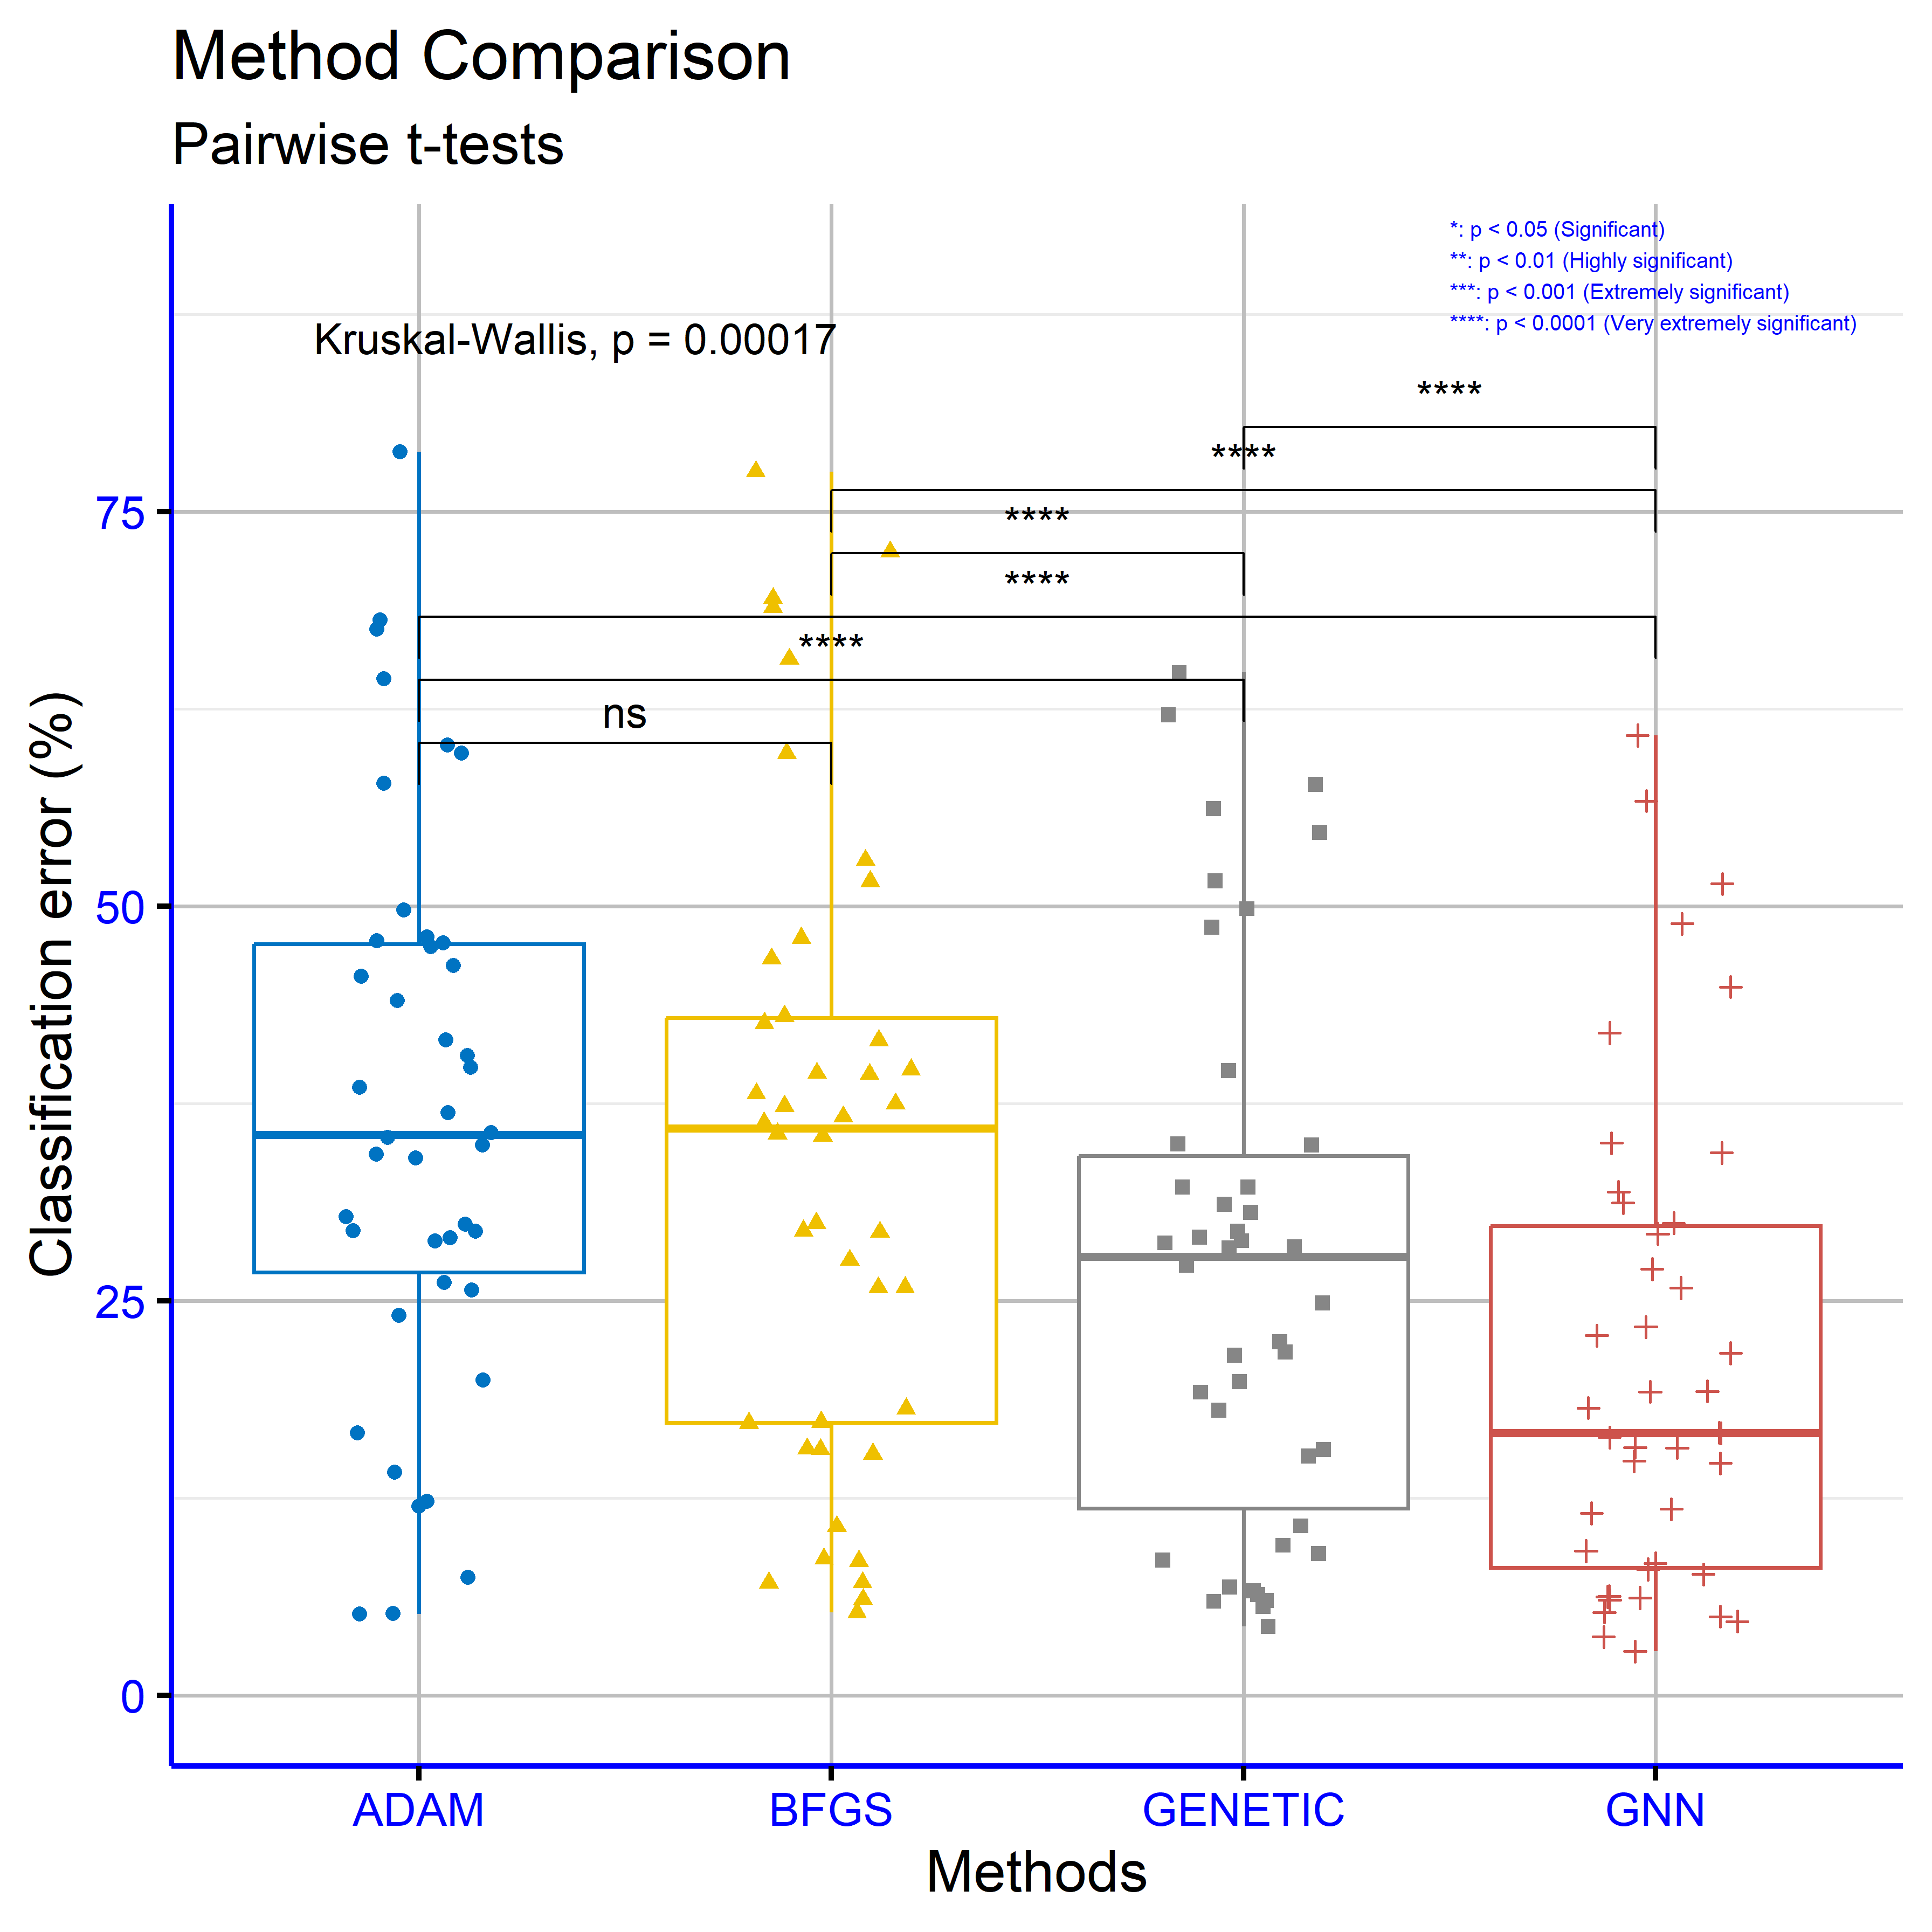
\includegraphics[scale=0.5]{stat1}
\par\end{centering}
\caption{Statistical comparison between the used methods for the classification
datasets.\label{fig:statClass}}

\end{figure}
\begin{figure}[H]
\begin{centering}
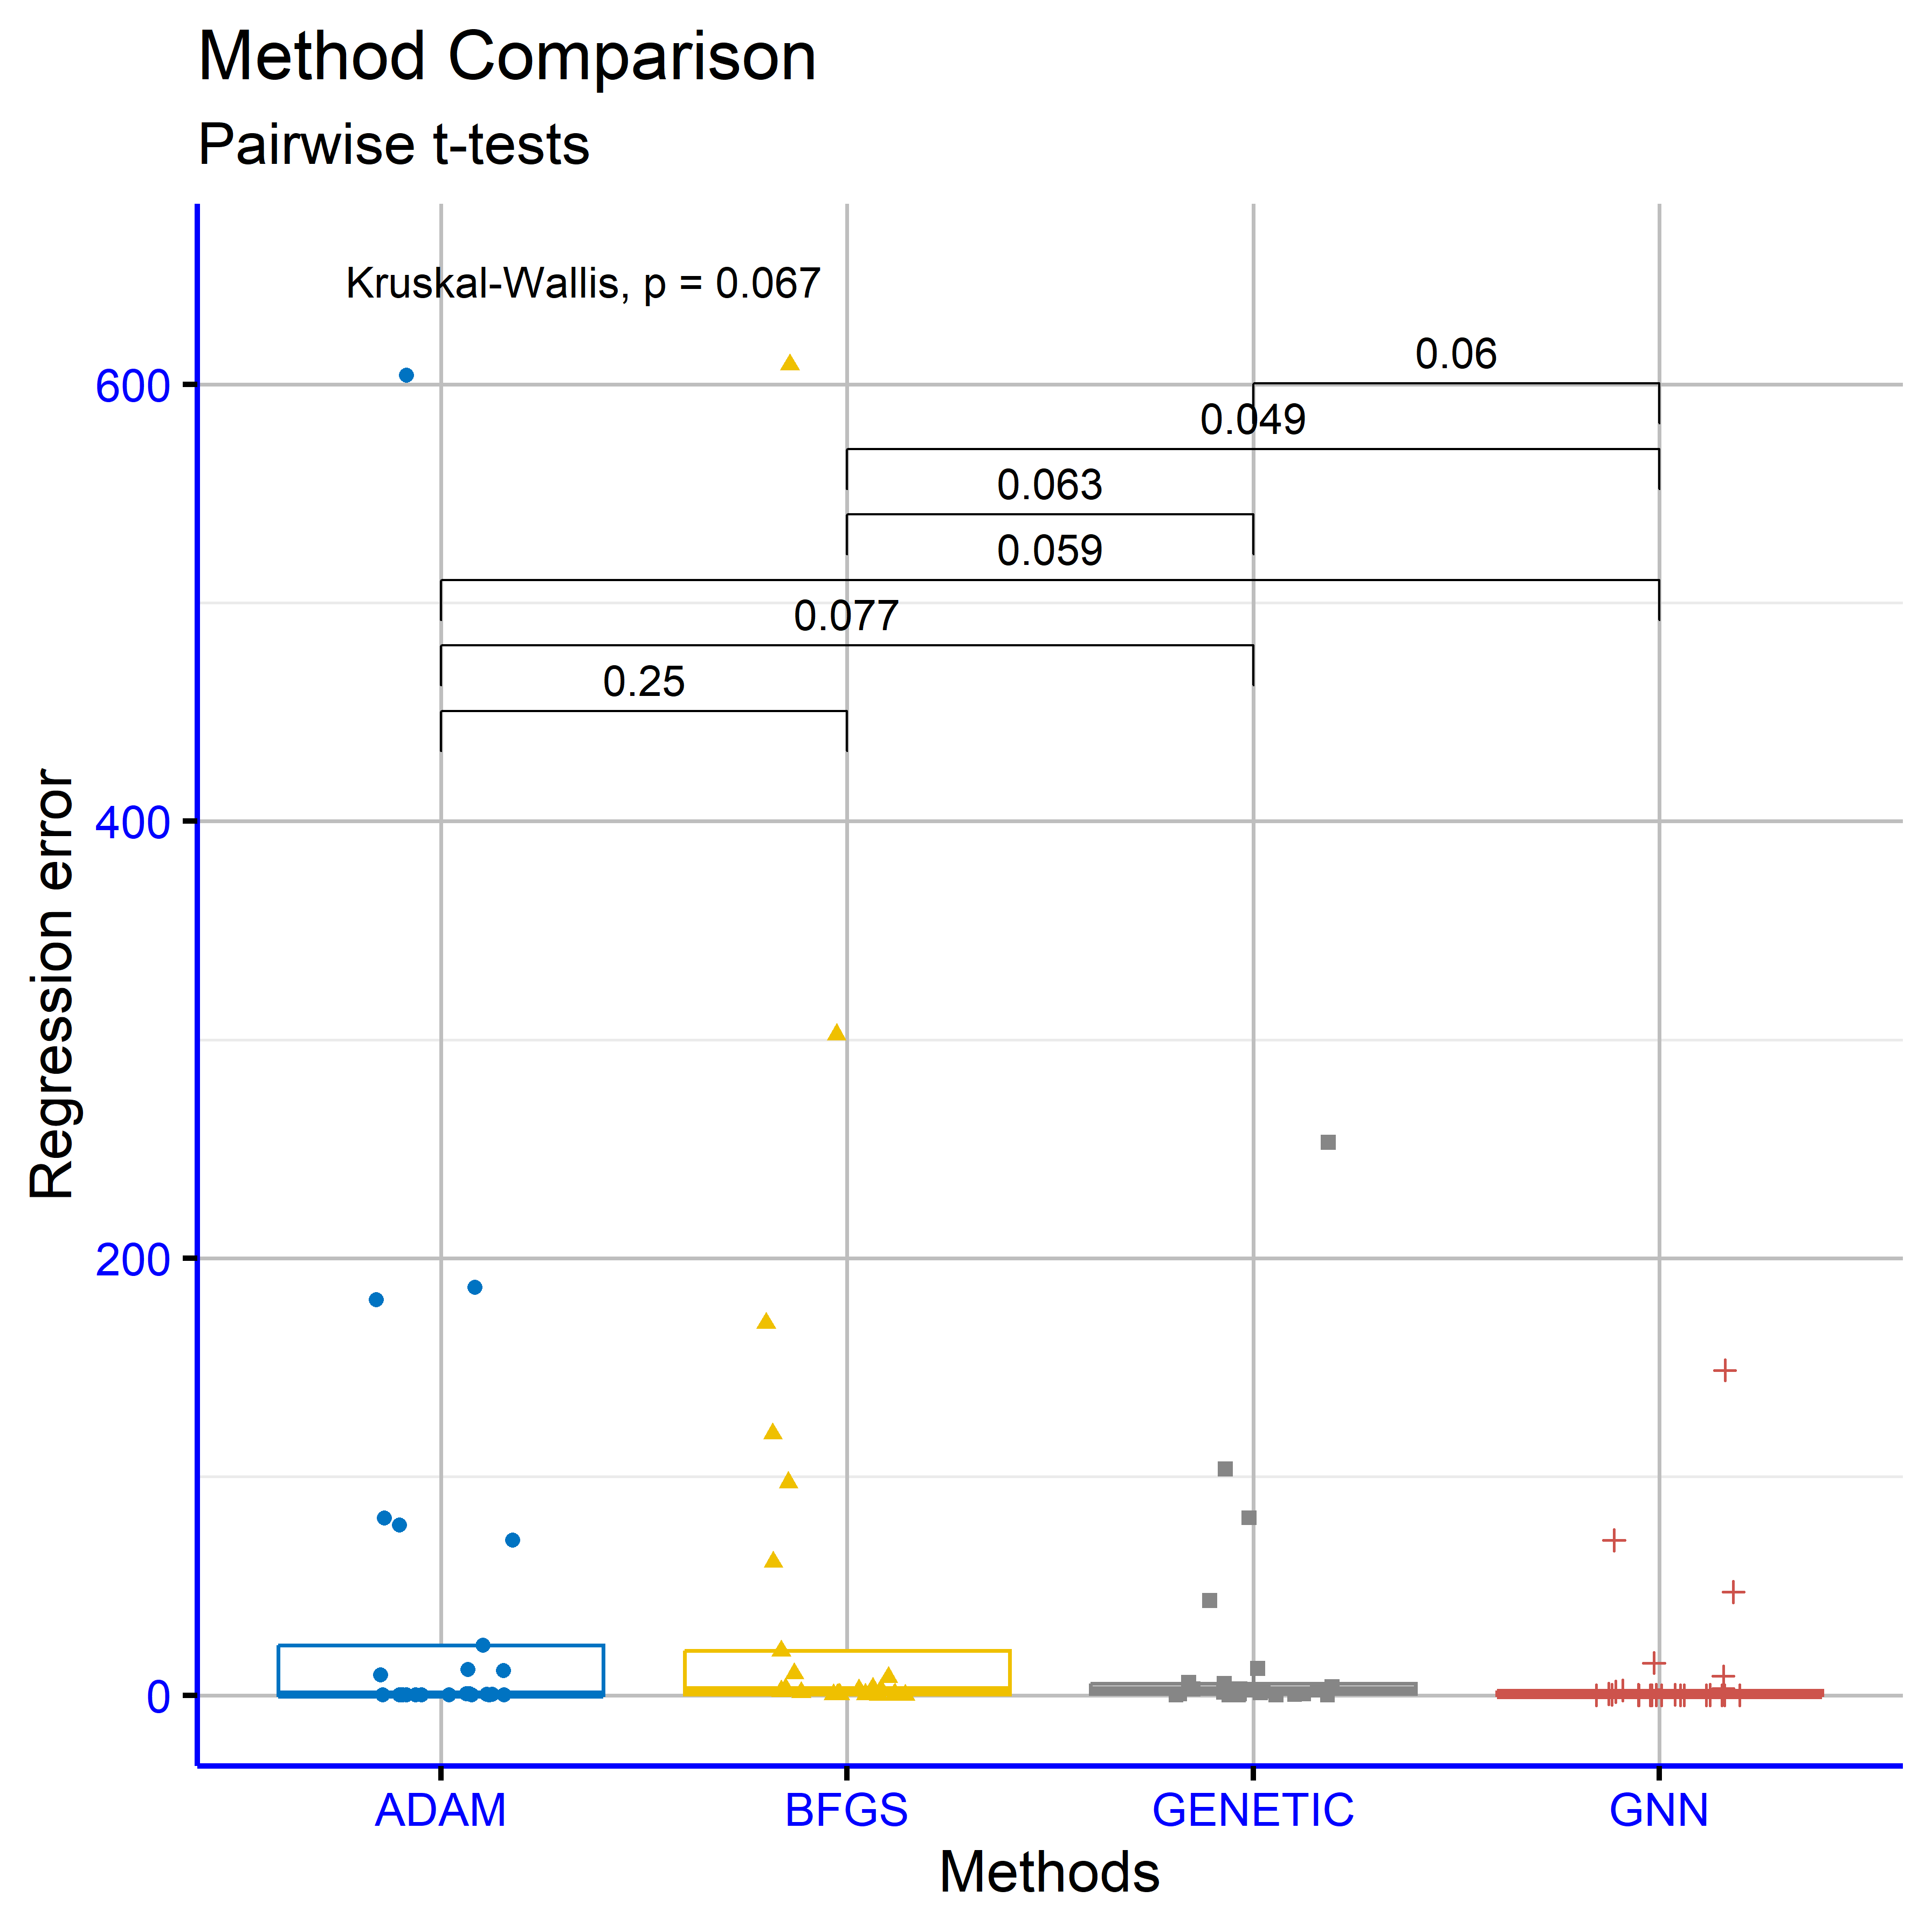
\includegraphics[scale=0.5]{stat2}
\par\end{centering}
\caption{Statistical comparison between the used methods for the regression
datasets.\label{fig:statRegression}}

\end{figure}

The statistical analysis conducted using the Wilcoxon Test (Figure
\ref{fig:statClass}) to compare the models from Table {[}table3{]}
reveals significant differences in performance, as evidenced by the
extremely low p-values. The p-value is an indicator of the probability
that the observed differences in performance between models are due
to random factors, with values below the conventional threshold (e.g.,
0.05) being considered statistically significant. In this analysis,
all p-values are exceptionally low, indicating that the differences
between GNN and the other models are statistically robust. The comparison
between GNN and ADAM yielded a p-value of 9.1e-13, indicating that
the probability of the observed differences being random is nearly
zero. This result highlights the clear superiority of GNN over ADAM.
Similarly, the p-value of 2e-11 for the comparison between GNN and
BFGS demonstrates that GNN achieves significantly lower errors than
BFGS, confirming the latter's inferior performance. The analysis of
the pairs GNN and GENETIC (p = 5.2e-09) and GNN and NEAT (p = 5.7e-10)
indicates that although the GENETIC and NEAT models have specific
strengths in individual datasets, their overall performance does not
approach that of GNN. The differences are statistically significant,
clearly establishing GNN as the superior choice under the conditions
examined. Lastly, the comparison between GNN and RBF (p = 1.8e-08)
demonstrates that GNN also outperforms RBF, despite RBF showing strong
results in selected datasets. This analysis provides a comprehensive
view of GNN's superiority, not only in terms of average error but
also from a statistical perspective, confirming that the performance
differences are not products of random variations in the data. This
substantial differentiation underscores the value of GNN as a particularly
effective model for classification problems and highlights the need
for further exploration of the structure and characteristics that
contribute to its performance. Moreover, it reinforces the importance
of applying statistical techniques such as the Wilcoxon Test to make
informed decisions when comparing different machine learning algorithms.

In Figure \ref{fig:statRegression}, the comparison between GNN and
ADAM yields a p-value of 0.0011, indicating that GNN demonstrates
significantly better performance than ADAM. Although this value is
higher than the others, it remains statistically significant, underscoring
GNN's superiority in terms of error rates. The difference between
GNN and BFGS is even more pronounced, with a p-value of 2.8e-07, signifying
that GNN outperforms BFGS with very high statistical power. The p-values
for the comparisons of GNN with the models GENETIC (p = 3.9e-05),
NEAT (p = 5.5e-05), and RBF (p = 0.013) further strengthen the evidence
of GNN’s superiority. While RBF appears to exhibit relatively better
performance than the other models compared with GNN, the p-value of
0.013 indicates that the difference is still statistically significant
and supports the preference for GNN. These results confirm GNN's superiority
in regression problems concerning its overall performance, suggesting
that the lower error rates it achieves are not due to random factors
but reflect its effectiveness. This analysis highlights the importance
of using statistical tools like the Wilcoxon Test to evaluate the
performance of machine learning algorithms and emphasizes the need
for a tailored model selection process, taking into account the specific
characteristics of each problem.

\section{Conclusions\label{sec:Conclusions}}

The article highlights a novel methodology for training artificial
neural networks using Backus-Naur Form grammars combined with Grammatical
Evolution. This approach provides a structured framework for defining
and optimizing neural network architectures, enhancing their adaptability
and performance across various problem domains. The proposed three-phase
process includes parameter specification, evolutionary optimization
of parameter bounds, and final training with specialized optimization
algorithms. The methodology demonstrates strong versatility and achieves
high performance across diverse architectures such as recurrent neural
networks and convolutional neural networks, handling both classification
and regression tasks effectively. The use of Backus-Naur Form grammars
constrains the parameter search space, reducing computational complexity
and mitigating risks associated with local minima or suboptimal solutions.
The experimental findings reveal that GNN outperforms traditional
optimization methods, including ADAM, BFGS, and GENETIC, consistently
achieving lower error rates. This result highlights the effectiveness
of the proposed method in initializing and optimizing network parameters.
GNN’s generalization capabilities and adaptability to different datasets
further underscore its potential in real-world applications requiring
precision and reliability. The results confirm that the lower error
rates achieved by GNN are not due to random factors but reflect the
robustness of the method. Future explorations could extend the methodology
to more complex deep learning architectures, including transformers
and graph neural networks, where the dimensionality and complexity
of parameters are significantly higher. Dynamic and non-stationary
environments such as real-time data streams and adaptive control systems
present another promising area of application. 

Incorporating the methodology into neural architecture search frameworks
could automate the discovery of optimal architectures, leveraging
Backus-Naur Form grammars to balance exploration and exploitation
efficiently. Multimodal data scenarios that combine textual, visual,
and auditory inputs could also benefit from this approach by enabling
hybrid architectures capable of processing diverse information types
effectively. Addressing scalability concerns through parallel and
distributed computing frameworks could enable the method to handle
large-scale datasets and complex architectures. Domain-specific grammars
tailored to particular problem types, such as time-series forecasting
or anomaly detection, could further refine the applicability and efficiency
of the method. Combining the evolutionary optimization process with
gradient-based techniques could provide a hybrid approach, enhancing
convergence speed while maintaining flexibility in exploring the parameter
space. 

Empirical studies across broader datasets and theoretical investigations
into the convergence properties and computational complexity of the
method would offer deeper insights into its strengths and limitations.
The methodology represents a significant advancement in neural network
training, offering robust adaptability and precision across diverse
applications. Its potential for scalability, domain-specific customizations,
and hybrid optimization approaches underscores its relevance for addressing
increasingly complex and dynamic challenges in machine learning.

$ $

\authorcontributions{V.C. and I.G.T. conducted the experiments, employing several datasets
and provided the comparative experiments. D.T. and V.C. performed
the statistical analysis and prepared the manuscript. All authors
have read and agreed to the published version of the manuscript.}

\funding{This research received no external funding.}

\institutionalreview{Not applicable.}

\informedconsent{Not applicable.}

\dataavailability{Not applicable.}

\acknowledgments{This research has been financed by the European Union : Next Generation
EU through the Program Greece 2.0 National Recovery and Resilience
Plan , under the call RESEARCH -- CREATE -- INNOVATE, project name
“iCREW: Intelligent small craft simulator for advanced crew training
using Virtual Reality techniques\textquotedbl{} (project code:TAEDK-06195).}

\conflictsofinterest{The authors declare no conflicts of interest.}

\begin{adjustwidth}{-\extralength}{0cm}{}

\reftitle{References}
\begin{thebibliography}{999}
\bibitem[(2006)]{physics-ml1} M. Mjahed, The use of clustering techniques
for the classification of high energy physics data, Nuclear Instruments
and Methods in Physics Research Section A: Accelerators, Spectrometers,
Detectors and Associated Equipment \textbf{559}, pp. 199-202, 2006.

\bibitem{physics_ml2}M Andrews, M Paulini, S Gleyzer, B Poczos, End-to-End
Event Classification of High-Energy Physics Data, Journal of Physics:
Conference Series \textbf{1085}, 2018.

\bibitem{chemistry_ml1}P. He, C.J. Xu, Y.Z. Liang, K.T. Fang, Improving
the classification accuracy in chemistry via boosting technique, Chemometrics
and Intelligent Laboratory Systems 70, pp. 39-46, 2004.

\bibitem{chemistry_ml2}J.A. Aguiar, M.L. Gong, T.Tasdizen, Crystallographic
prediction from diffraction and chemistry data for higher throughput
classification using machine learning, Computational Materials Science
\textbf{173}, 109409, 2020.

\bibitem{econ_ml1}I. Kaastra, M. Boyd, Designing a neural network
for forecasting financial and economic time series, Neurocomputing
\textbf{10}, pp. 215-236, 1996.

\bibitem{econ_ml2}R. Hafezi, J. Shahrabi, E. Hadavandi, A bat-neural
network multi-agent system (BNNMAS) for stock price prediction: Case
study of DAX stock price, Applied Soft Computing \textbf{29}, pp.
196-210, 2015.

\bibitem{med_ml1}S.S. Yadav, S.M. Jadhav, Deep convolutional neural
network based medical image classification for disease diagnosis.
J Big Data \textbf{6}, 113, 2019.

\bibitem{med_ml2}L. Qing, W. Linhong , D. Xuehai, A Novel Neural
Network-Based Method for Medical Text Classification, Future Internet
\textbf{11}, 255, 2019.

\bibitem{nn1}C. Bishop, Neural Networks for Pattern Recognition,
Oxford University Press, 1995.

\bibitem{nn2}G. Cybenko, Approximation by superpositions of a sigmoidal
function, Mathematics of Control Signals and Systems \textbf{2}, pp.
303-314, 1989.

\bibitem{nn_image}M. Egmont-Petersen, D. de Ridder, H. Handels, Image
processing with neural networks---a review, Pattern recognition \textbf{35},
pp. 2279-2301, 2002.

\bibitem{nn-times}M. Khashei, M. Bijari, An artificial neural network
(p,d,q) model for timeseries forecasting, Expert Systems with Applications
\textbf{37}, pp. 479-489, 2010.

\bibitem{nn_solar}A. Mellit, A. Massi Pavan, A 24-h forecast of solar
irradiance using artificial neural network: Application for performance
prediction of a grid-connected PV plant at Trieste, Italy, Solar Energy
\textbf{84}, pp. 807-821, 2010.

\bibitem{nn_medical}F. Amato, A. López, E. María Peña-Méndez, P.
Vaňhara,A. Hampl, J. Havel, Artificial neural networks in medical
diagnosis, Journal of Applied Biomedicine \textbf{11}, pp. 47-58,
2013.

\bibitem{nnde1}Y. Shirvany, M. Hayati, R. Moradian, Multilayer perceptron
neural networks with novel unsupervised training method for numerical
solution of the partial differential equations, Applied Soft Computing
\textbf{9}, pp. 20-29, 2009.

\bibitem{nnde2}A. Malek, R. Shekari Beidokhti, Numerical solution
for high order differential equations using a hybrid neural network---Optimization
method, Applied Mathematics and Computation \textbf{183}, pp. 260-271,
2006.

\bibitem{nnagr1}A. Topuz, Predicting moisture content of agricultural
products using artificial neural networks, Advances in Engineering
Software \textbf{41}, pp. 464-470, 2010.

\bibitem{nnagr2}A. Escamilla-García, G.M. Soto-Zarazúa, M. Toledano-Ayala,
E. Rivas-Araiza, A. Gastélum-Barrios, Abraham,Applications of Artificial
Neural Networks in Greenhouse Technology and Overview for Smart Agriculture
Development, Applied Sciences \textbf{10}, Article number 3835, 2020.

\bibitem{bpnn}D.E. Rumelhart, G.E. Hinton and R.J. Williams, Learning
representations by back-propagating errors, Nature \textbf{323}, pp.
533 - 536 , 1986.

\bibitem{rpropnn-1}M. Riedmiller and H. Braun, A Direct Adaptive
Method for Faster Backpropagation Learning: The RPROP algorithm, Proc.
of the IEEE Intl. Conf. on Neural Networks, San Francisco, CA, pp.
586--591, 1993.

\bibitem{Adam}D. P. Kingma, J. L. Ba, ADAM: a method for stochastic
optimization, in: Proceedings of the 3rd International Conference
on Learning Representations (ICLR 2015), pp. 1--15, 2015.

\bibitem{quasinn}B. Robitaille and B. Marcos and M. Veillette and
G. Payre, Modified quasi-Newton methods for training neural networks,
Computers \& Chemical Engineering \textbf{20}, pp. 1133-1140, 1996.

\bibitem{tabunn}R.S. Sexton, B. Alidaee, R.E. Dorsey, J.D. Johnson,
Global optimization for artificial neural networks: A tabu search
application. European Journal of Operational Research \textbf{106},
pp. 570-584, 1998.

\bibitem{nn_ann1}A. Yamazaki, M. C. P. de Souto,T. B. Ludermir, Optimization
of neural network weights and architectures for odor recognition using
simulated annealing, In: Proceedings of the 2002 International Joint
Conference on Neural Networks. IJCNN'02 \textbf{1}, pp. 547-552 ,
2002.

\bibitem{geneticnn}F. H. F. Leung, H. K. Lam, S. H. Ling and P. K.
S. Tam, Tuning of the structure and parameters of a neural network
using an improved genetic algorithm, IEEE Transactions on Neural Networks
\textbf{14}, pp. 79-88, 2003

\bibitem{psonn}C. Zhang, H. Shao and Y. Li, Particle swarm optimization
for evolving artificial neural network, IEEE International Conference
on Systems, Man, and Cybernetics, , pp. 2487-2490, 2000.

\bibitem{weight_de1}J. lonen, J.K. Kamarainen, J. Lampinen, Differential
Evolution Training Algorithm for Feed-Forward Neural Networks, Neural
Processing Letters \textbf{17}, pp. 93--105, 2003.

\bibitem{weight_aco}K.M. Salama, A.M. Abdelbar, Learning neural network
structures with ant colony algorithms, Swarm Intell \textbf{9}, pp.
229--265, 2015.

\bibitem{weight_bmo}A. Askarzadeh, A. Rezazadeh, Artificial neural
network training using a new efficient optimization algorithm, Applied
Soft Computing \textbf{13}, pp. 1206-1213, 2013.

\bibitem{weight_arch}P.G. Benardos, G.-C. Vosniakos, Optimizing feedforward
artificial neural network architecture, Engineering Applications of
Artificial Intelligence \textbf{20}, pp. 365-382, 2007.

\bibitem{weight_abc}D. Karaboga and B. Akay, \textquotedbl Artificial
Bee Colony (ABC) Algorithm on Training Artificial Neural Networks,\textquotedbl{}
2007 IEEE 15th Signal Processing and Communications Applications,
Eskisehir, Turkey, 2007, pp. 1-4, doi: 10.1109/SIU.2007.4298679.

\bibitem{nnhybrid2}J.F. Chen, Q.H. Do,H.N. Hsieh, Training Artificial
Neural Networks by a Hybrid PSO-CS Algorithm, Algorithms \textbf{8},
pp. 292-308, 2015.

\bibitem{csmethod}X.S. Yang, S. Deb, Engineering Optimisation by
Cuckoo Search, Int. J. Math. Model. Numer. Optim. \textbf{1}, 330--343,
2010.

\bibitem{nnpar1}S. Scanzio, S. Cumani, R. Gemello, F. Mana, P. Laface,
Parallel implementation of Artificial Neural Network training for
speech recognition, Pattern Recognition Letters \textbf{31}, pp. 1302-1309,
2010.

\bibitem{nnpar2}X. Sierra-Canto, F. Madera-Ramirez and V. Uc-Cetina,
\textquotedbl Parallel Training of a Back-Propagation Neural Network
Using CUDA,\textquotedbl{} 2010 Ninth International Conference on
Machine Learning and Applications, Washington, DC, USA, 2010, pp.
307-312, doi: 10.1109/ICMLA.2010.52.

\bibitem{nnpar3}F. Åström, R. Koker, A parallel neural network approach
to prediction of Parkinson’s Disease, Expert Systems with Applications
\textbf{38}, , pp. 12470-12474, 2011.

\bibitem{nninit1}I. Ivanova, M. Kubat, Initialization of neural networks
by means of decision trees, Knowledge-Based Systems \textbf{8}, pp.
333-344, 1995.

\bibitem{weight_init2}J.Y.F. Yam, T.W.S. Chow, A weight initialization
method for improving training speed in feedforward neural network,
Neurocomputing \textbf{30}, pp. 219-232, 2000.

\bibitem{weight_init3}K. Chumachenko, A. Iosifidis, M. Gabbouj, Feedforward
neural networks initialization based on discriminant learning, Neural
Networks \textbf{146}, pp. 220-229, 2022.

\bibitem{nninit2}F. Itano, M. A. de Abreu de Sousa, E. Del-Moral-Hernandez,
Extending MLP ANN hyper-parameters Optimization by using Genetic Algorithm,
In: 2018 International Joint Conference on Neural Networks (IJCNN),
Rio de Janeiro, Brazil, 2018, pp. 1-8, 2018.

\bibitem{nninit_interval}S.S. Sodhi, P. Chandra, Interval based Weight
Initialization Method for Sigmoidal Feedforward Artificial Neural
Networks, AASRI Procedia \textbf{6}, pp. 19-25, 2014.

\bibitem{nninit_overview}C. A. R. de Sousa, \textquotedbl An overview
on weight initialization methods for feedforward neural networks,\textquotedbl{}
2016 International Joint Conference on Neural Networks (IJCNN), Vancouver,
BC, Canada, 2016, pp. 52-59, doi: 10.1109/IJCNN.2016.7727180.

\bibitem{nnsharing1}S.J. Nowlan and G.E. Hinton, Simplifying neural
networks by soft weight sharing, Neural Computation 4, pp. 473-493,
1992.

\bibitem{nnprunning1}S.J. Hanson and L.Y. Pratt, Comparing biases
for minimal network construction with back propagation, In D.S. Touretzky
(Ed.), Advances in Neural Information Processing Systems, Volume 1,
pp. 177-185, San Mateo, CA: Morgan Kaufmann, 1989.

\bibitem{nnprunning2}M.C. Mozer and P. Smolensky, Skeletonization:
a technique for trimming the fat from a network via relevance assesment.
In D.S. Touretzky (Ed.), Advances in Neural Processing Systems, Volume
1, pp. 107-115, San Mateo CA: Morgan Kaufmann, 1989.

\bibitem{nnprunning3}M. Augasta and T. Kathirvalavakumar, Pruning
algorithms of neural networks --- a comparative study, Central European
Journal of Computer Science, 2003.

\bibitem{nndrop1}Nitish Srivastava, G E Hinton, Alex Krizhevsky,
Ilya Sutskever, Ruslan R Salakhutdinov, Dropout: a simple way to prevent
neural networks from overfitting, Journal of Machine Learning Research
\textbf{15}, pp. 1929-1958, 2014.

\bibitem{nndecay1}A. Gupta, S.M. Lam, Weight decay backpropagation
for noisy data, Neural Networks \textbf{11}, pp. 1127-1138, 1998.

\bibitem{nndecay2}M. Carvalho and T. B. Ludermir, Particle Swarm
Optimization of Feed-Forward Neural Networks with Weight Decay, 2006
Sixth International Conference on Hybrid Intelligent Systems (HIS'06),
Rio de Janeiro, Brazil, 2006, pp. 5-5.

\bibitem{sarprop}N.K. Treadgold, T.D. Gedeon, Simulated annealing
and weight decay in adaptive learning: the SARPROP algorithm, IEEE
Trans. on Neural Networks 9, pp. 662-668, 1998.

\bibitem{nnpositive}M.D. Shahjahan, M. Kazuyuki, Neural network training
algorithm with possitive correlation, IEEE Trans. Inf \& Syst. \textbf{88},
pp. 2399-2409, 2005.

\bibitem{gen_review}Mirjalili, S., \& Mirjalili, S. (2019). Genetic
algorithm. Evolutionary algorithms and neural networks: theory and
applications, 43-55.

\bibitem{mainge}M. O’Neill, C. Ryan, Grammatical evolution, IEEE
Trans. Evol. Comput. \textbf{5,}pp. 349--358, 2001.

\bibitem{rnn1}M. Lukoševičius, H. Jaeger, Reservoir computing approaches
to recurrent neural network training, Computer science review \textbf{3},
pp. 127-149, 2009.

\bibitem{cnn1}J. Gu, Z. Wang, J. Kuen, L. Ma, A. Shahroudy, B. Shuai,
T. Chen, Recent advances in convolutional neural networks, Pattern
recognition\textbf{ 77}, pp. 354-377, 2018.

\bibitem{bnf1}J. W. Backus. The Syntax and Semantics of the Proposed
International Algebraic Language of the Zurich ACM-GAMM Conference.
Proceedings of the International Conference on Information Processing,
UNESCO, 1959, pp.125-132.

\bibitem[(1991)]{ge_music}A.O. Puente, R. S. Alfonso, M. A. Moreno,
Automatic composition of music by means of grammatical evolution,
In: APL '02: Proceedings of the 2002 conference on APL: array processing
languages: lore, problems, and applications July 2002 Pages 148--155. 

\bibitem[(1991)]{ge_pacman}E. Galván-López, J.M. Swafford, M. O’Neill,
A. Brabazon, Evolving a Ms. PacMan Controller Using Grammatical Evolution.
In: , et al. Applications of Evolutionary Computation. EvoApplications
2010. Lecture Notes in Computer Science, vol 6024. Springer, Berlin,
Heidelberg, 2010.

\bibitem{ge_supermario}N. Shaker, M. Nicolau, G. N. Yannakakis, J.
Togelius, M. O'Neill, Evolving levels for Super Mario Bros using grammatical
evolution, 2012 IEEE Conference on Computational Intelligence and
Games (CIG), 2012, pp. 304-31.

\bibitem{ge_fractal}A. Ortega, A. A. Dalhoum, M. Alfonseca, Grammatical
evolution to design fractal curves with a given dimension, IBM Journal
of Research and Development \textbf{47}, pp. 483-493, 2003.

\bibitem{ge_constant}I. Dempsey, M.O' Neill, A. Brabazon, Constant
creation in grammatical evolution, International Journal of Innovative
Computing and Applications \textbf{1} , pp 23--38, 2007.

\bibitem{ge_robot}R. Burbidge, J. H. Walker and M. S. Wilson, \textquotedbl Grammatical
evolution of a robot controller,\textquotedbl{} 2009 IEEE/RSJ International
Conference on Intelligent Robots and Systems, St. Louis, MO, USA,
2009, pp. 357-362, doi: 10.1109/IROS.2009.5354411.

\bibitem{ge_robotics}Peabody, C., \& Seitzer, J. (2015, March). GEF:
a self-programming robot using grammatical evolution. In Proceedings
of the AAAI Conference on Artificial Intelligence (Vol. 29, No. 1).

\bibitem{ge_glykemia}J. I. Hidalgo, J. M. Colmenar, J.L. Risco-Martin,
A. Cuesta-Infante, E. Maqueda, M. Botella, J.A. Rubio, Modeling glycemia
in humans by means of Grammatical Evolution, Applied Soft Computing
\textbf{20}, pp. 40-53, 2014.

\bibitem{ge_wikipedia}L. Araujo, J. Martinez-Romo, A. Duque, Discovering
taxonomies in Wikipedia by means of grammatical evolution. Soft Comput
\textbf{22}, pp. 2907--2919, 2018. 

\bibitem{ge_trading}C. Martín, D. Quintana, P. Isasi, Grammatical
Evolution-based ensembles for algorithmic trading, Applied Soft Computing
\textbf{84}, 105713, 2019.

\bibitem{nnc}I.G. Tsoulos, D. Gavrilis, E. Glavas, Neural network
construction and training using grammatical evolution, Neurocomputing
\textbf{72}, pp. 269-277, 2008.

\bibitem{kaelo}P. Kaelo, M.M. Ali, Integrated crossover rules in
real coded genetic algorithms, European Journal of Operational Research
\textbf{176}, pp. 60-76, 2007.

\bibitem{powell}M.J.D Powell, A Tolerant Algorithm for Linearly Constrained
Optimization Calculations, Mathematical Programming \textbf{45}, pp.
547-566, 1989. 

\bibitem[(1989)]{uci} M. Kelly, R. Longjohn, K. Nottingham, The UCI
Machine Learning Repository, https://archive.ics.uci.edu.

\bibitem{Keel}J. Alcalá-Fdez, A. Fernandez, J. Luengo, J. Derrac,
S. García, L. Sánchez, F. Herrera. KEEL Data-Mining Software Tool:
Data Set Repository, Integration of Algorithms and Experimental Analysis
Framework. Journal of Multiple-Valued Logic and Soft Computing 17,
pp. 255-287, 2011.

\bibitem[Tzimourta(2018)]{alcohol}Tzimourta, K.D.; Tsoulos, I.; Bilero,
I.T.; Tzallas, A.T.; Tsipouras, M.G.; Giannakeas, N. Direct Assessment
of Alcohol Consumption in Mental State Using Brain Computer Interfaces
and Grammatical Evolution. Inventions 2018, 3, 51.

\bibitem[Quinlan(2018)]{australian}J.R. Quinlan, Simplifying Decision
Trees. International Journal of Man-Machine Studies \textbf{27}, pp.
221-234, 1987. 

\bibitem[Evans(1994)]{bands}B. Evans, D. Fisher, Overcoming process
delays with decision tree induction. IEEE Expert \textbf{9}, pp. 60-66,
1994.

\bibitem[(2004)]{cleveland1}Z.H. Zhou,Y. Jiang, NeC4.5: neural ensemble
based C4.5,\textquotedbl{} in IEEE Transactions on Knowledge and Data
Engineering \textbf{16}, pp. 770-773, 2004.

\bibitem{cleveland2}R. Setiono , W.K. Leow, FERNN: An Algorithm for
Fast Extraction of Rules from Neural Networks, Applied Intelligence
\textbf{12}, pp. 15-25, 2000.

\bibitem[(1998)]{dermatology}G. Demiroz, H.A. Govenir, N. Ilter,
Learning Differential Diagnosis of Eryhemato-Squamous Diseases using
Voting Feature Intervals, Artificial Intelligence in Medicine. \textbf{13},
pp. 147--165, 1998.

\bibitem[(1996)]{ecoli}P. Horton, K.Nakai, A Probabilistic Classification
System for Predicting the Cellular Localization Sites of Proteins,
In: Proceedings of International Conference on Intelligent Systems
for Molecular Biology \textbf{4}, pp. 109-15, 1996.

\bibitem[(1977)]{hayes-roth}B. Hayes-Roth, B., F. Hayes-Roth. Concept
learning and the recognition and classification of exemplars. Journal
of Verbal Learning and Verbal Behavior \textbf{16}, pp. 321-338, 1977.

\bibitem[(1997)]{heart}I. Kononenko, E. Šimec, M. Robnik-Šikonja,
Overcoming the Myopia of Inductive Learning Algorithms with RELIEFF,
Applied Intelligence \textbf{7}, pp. 39--55, 1997

\bibitem[(2002)]{housevotes}R.M. French, N. Chater, Using noise to
compute error surfaces in connectionist networks: a novel means of
reducing catastrophic forgetting, Neural Comput. \textbf{14}, pp.
1755-1769, 2002.

\bibitem[(2004)]{ion1}J.G. Dy , C.E. Brodley, Feature Selection for
Unsupervised Learning, The Journal of Machine Learning Research \textbf{5},
pp 845--889, 2004.

\bibitem{ion2}S. J. Perantonis, V. Virvilis, Input Feature Extraction
for Multilayered Perceptrons Using Supervised Principal Component
Analysis, Neural Processing Letters \textbf{10}, pp 243--252, 1999.

\bibitem[(2002)]{liver} J. Garcke, M. Griebel, Classification with
sparse grids using simplicial basis functions, Intell. Data Anal.
\textbf{6}, pp. 483-502, 2002.

\bibitem{liver1}J. Mcdermott, R.S. Forsyth, Diagnosing a disorder
in a classification benchmark, Pattern Recognition Letters \textbf{73},
pp. 41-43, 2016.

\bibitem[(2002)]{lymography}G. Cestnik, I. Konenenko, I. Bratko,
Assistant-86: A Knowledge-Elicitation Tool for Sophisticated Users.
In: Bratko, I. and Lavrac, N., Eds., Progress in Machine Learning,
Sigma Press, Wilmslow, pp. 31-45, 1987. 

\bibitem[(2002)]{magic}Heck, D., Knapp, J., Capdevielle, J. N., Schatz,
G., \& Thouw, T. (1998). CORSIKA: A Monte Carlo code to simulate extensive
air showers.

\bibitem[(2007)]{mammographic}M. Elter, R. Schulz-Wendtland, T. Wittenberg,
The prediction of breast cancer biopsy outcomes using two CAD approaches
that both emphasize an intelligible decision process, Med Phys. \textbf{34},
pp. 4164-72, 2007.

\bibitem[(2007)]{parkinsons1}M.A. Little, P.E. McSharry, S.J Roberts
et al, Exploiting Nonlinear Recurrence and Fractal Scaling Properties
for Voice Disorder Detection. BioMed Eng OnLine \textbf{6}, 23, 2007.

\bibitem{parkinsons2}M.A. Little, P.E. McSharry, E.J. Hunter, J.
Spielman, L.O. Ramig, Suitability of dysphonia measurements for telemonitoring
of Parkinson's disease. IEEE Trans Biomed Eng. \textbf{56}, pp. 1015-1022,
2009.

\bibitem[(2007)]{pima}J.W. Smith, J.E. Everhart, W.C. Dickson, W.C.
Knowler, R.S. Johannes, Using the ADAP learning algorithm to forecast
the onset of diabetes mellitus, In: Proceedings of the Symposium on
Computer Applications and Medical Care IEEE Computer Society Press,
pp.261-265, 1988.

\bibitem{pageblocks}F. Esposito F., D. Malerba, G. Semeraro, Multistrategy
Learning for Document Recognition, Applied Artificial Intelligence
\textbf{8}, pp. 33-84, 1994. 

\bibitem[(2007)]{popfailures}D.D. Lucas, R. Klein, J. Tannahill,
D. Ivanova, S. Brandon, D. Domyancic, Y. Zhang, Failure analysis of
parameter-induced simulation crashes in climate models, Geoscientific
Model Development \textbf{6}, pp. 1157-1171, 2013.

\bibitem[(2007)]{regions2}N. Giannakeas, M.G. Tsipouras, A.T. Tzallas,
K. Kyriakidi, Z.E. Tsianou, P. Manousou, A. Hall, E.C. Karvounis,
V. Tsianos, E. Tsianos, A clustering based method for collagen proportional
area extraction in liver biopsy images (2015) Proceedings of the Annual
International Conference of the IEEE Engineering in Medicine and Biology
Society, EMBS, 2015-November, art. no. 7319047, pp. 3097-3100. 

\bibitem[(2007)]{saheart}T. Hastie, R. Tibshirani, Non-parametric
logistic and proportional odds regression, JRSS-C (Applied Statistics)
\textbf{36}, pp. 260--276, 1987.

\bibitem{segment}M. Dash, H. Liu, P. Scheuermann, K. L. Tan, Fast
hierarchical clustering and its validation, Data \& Knowledge Engineering
\textbf{44}, pp 109--138, 2003.

\bibitem[(2007)]{student}P. Cortez, A. M. Gonçalves Silva, Using
data mining to predict secondary school student performance, In Proceedings
of 5th FUture BUsiness TEChnology Conference (FUBUTEC 2008) (pp. 5--12).
EUROSIS-ETI, 2008.

\bibitem[(2007)]{transfusion}I-Cheng Yeh, King-Jang Yang, Tao-Ming
Ting, Knowledge discovery on RFM model using Bernoulli sequence, Expert
Systems with Applications \textbf{36}, pp. 5866-5871, 2009.

\bibitem[(2007)]{wdbc1}Jeyasingh, S., \& Veluchamy, M. (2017). Modified
bat algorithm for feature selection with the wisconsin diagnosis breast
cancer (WDBC) dataset. Asian Pacific journal of cancer prevention:
APJCP, 18(5), 1257.

\bibitem[(2007)]{wdbc2}Alshayeji, M. H., Ellethy, H., \& Gupta, R.
(2022). Computer-aided detection of breast cancer on the Wisconsin
dataset: An artificial neural networks approach. Biomedical signal
processing and control, 71, 103141.

\bibitem[(2007)]{wine1}M. Raymer, T.E. Doom, L.A. Kuhn, W.F. Punch,
Knowledge discovery in medical and biological datasets using a hybrid
Bayes classifier/evolutionary algorithm. IEEE transactions on systems,
man, and cybernetics. Part B, Cybernetics : a publication of the IEEE
Systems, Man, and Cybernetics Society, \textbf{33} , pp. 802-813,
2003.

\bibitem{wine2}P. Zhong, M. Fukushima, Regularized nonsmooth Newton
method for multi-class support vector machines, Optimization Methods
and Software \textbf{22}, pp. 225-236, 2007.

\bibitem[(2007)]{eeg1}R. G. Andrzejak, K. Lehnertz, F.Mormann, C.
Rieke, P. David, and C. E. Elger, “Indications of nonlinear deterministic
and finite-dimensional structures in time series of brain electrical
activity: dependence on recording region and brain state,” Physical
Review E, vol. 64, no. 6, Article ID 061907, 8 pages, 2001. 

\bibitem{eeg2}A. T. Tzallas, M. G. Tsipouras, and D. I. Fotiadis,
“Automatic Seizure Detection Based on Time-Frequency Analysis and
Artificial Neural Networks,” Computational Intelligence and Neuroscience,
vol. 2007, Article ID 80510, 13 pages, 2007. doi:10.1155/2007/80510

\bibitem[(2007)]{zoo}M. Koivisto, K. Sood, Exact Bayesian Structure
Discovery in Bayesian Networks, The Journal of Machine Learning Research\textbf{
5}, pp. 549--573, 2004.

\bibitem[(2007)]{abalone}Nash, W.J.; Sellers, T.L.; Talbot, S.R.;
Cawthor, A.J.; Ford, W.B. The Population Biology of Abalone (\_Haliotis\_
species) in Tasmania. I. Blacklip Abalone (\_H. rubra\_) from the
North Coast and Islands of Bass Strait, Sea Fisheries Division; Technical
Report No. 48; Department of Primary Industry and Fisheries, Tasmania:
Hobart, Australia, 1994; ISSN 1034-3288

\bibitem[(2007)]{airfoil}Brooks, T.F.; Pope, D.S.; Marcolini, A.M.
Airfoil Self-Noise and Prediction. Technical Report, NASA RP-1218.
July 1989. Available online: https://ntrs.nasa.gov/citations/19890016302
(accessed on 14 November 2024).

\bibitem[(2007)]{concrete}I.Cheng Yeh, Modeling of strength of high
performance concrete using artificial neural networks, Cement and
Concrete Research. \textbf{28}, pp. 1797-1808, 1998. 

\bibitem{friedman}Friedman, J. (1991): Multivariate Adaptative Regression
Splines. Annals of Statistics, 19:1, 1-{}-141. 

\bibitem[(2007)]{housing}D. Harrison and D.L. Rubinfeld, Hedonic
prices and the demand for clean ai, J. Environ. Economics \& Management
\textbf{5}, pp. 81-102, 1978.

\bibitem{neat}K. O. Stanley, R. Miikkulainen, Evolving Neural Networks
through Augmenting Topologies, Evolutionary Computation \textbf{10},
pp. 99-127, 2002.

\bibitem[(1991)]{rbf1}J. Park and I. W. Sandberg, Universal Approximation
Using Radial-Basis-Function Networks, Neural Computation \textbf{3},
pp. 246-257, 1991.

\bibitem{rbf2}G.A. Montazer, D. Giveki, M. Karami, H. Rastegar, Radial
basis function neural networks: A review. Comput. Rev. J \textbf{1},
pp. 52-74, 2018.

\end{thebibliography}

\end{adjustwidth}{}
\end{document}
